% =====================================================================
% Card upgrade recommendation engine -- end-to-end approach report
% Compile:  pdflatex report.tex   (run twice for the table of contents)
% Self-contained: every diagram and chart is drawn with TikZ / pgfplots
% from numbers read out of the actual pipeline outputs (data/*.parquet).
% =====================================================================
\documentclass[11pt,a4paper]{article}

\usepackage[T1]{fontenc}
\usepackage[utf8]{inputenc}
\usepackage{lmodern}
\usepackage[a4paper,margin=2.2cm]{geometry}
\usepackage{microtype}
\usepackage{amsmath,amssymb}
\usepackage{booktabs,tabularx,array}
\usepackage[table]{xcolor}
\usepackage{enumitem}
\usepackage{float}
\usepackage{needspace}
\usepackage{caption}
\usepackage{fancyhdr}
\usepackage{tikz}
\usepackage{pgfplots}
\usepackage{pgfplotstable}
\usepgfplotslibrary{groupplots}
\usetikzlibrary{arrows.meta,positioning,shapes.geometric,fit,calc,backgrounds}
\usepackage[most]{tcolorbox}
\usepackage[colorlinks=true,linkcolor=blue!50!black,urlcolor=blue!50!black]{hyperref}

\pgfplotsset{compat=1.18}

% ---------- palette ----------
\definecolor{cb}{HTML}{3B6EA8}   % baseline
\definecolor{ct}{HTML}{2E8B57}   % transactor
\definecolor{cr}{HTML}{C0392B}   % revolver
\definecolor{ca}{HTML}{E08E0B}   % accent
\definecolor{cg}{HTML}{6C757D}   % grey
\definecolor{cp}{HTML}{7D5BA6}   % purple
\definecolor{ck}{HTML}{17A2B8}   % teal

% ---------- helpers ----------
\newcommand{\eur}{\texttt{\texteuro}}
\newcommand{\code}[1]{\texttt{\detokenize{#1}}}
\newcommand{\why}[1]{\par\needspace{6\baselineskip}\smallskip\noindent\textbf{\textcolor{ca}{Why.}} #1\par}
\newcommand{\pt}{\,\text{pt}}

\setlist{itemsep=2pt,topsep=4pt}
\captionsetup{font=small,labelfont=bf}
\setlength{\parindent}{0pt}
\setlength{\parskip}{5pt}
\pagestyle{fancy}\fancyhf{}
\fancyhead[L]{\small Card upgrade recommendation engine}
\fancyhead[R]{\small End-to-end approach}
\fancyfoot[C]{\small\thepage}
\renewcommand{\headrulewidth}{0.3pt}

\newtcolorbox{keybox}[1][]{enhanced,breakable,colback=blue!4,colframe=cb!70!black,
  boxrule=0.5pt,arc=2pt,left=6pt,right=6pt,top=4pt,bottom=4pt,#1}
\newtcolorbox{warnbox}[1][]{enhanced,breakable,colback=orange!6,colframe=ca!90!black,
  boxrule=0.5pt,arc=2pt,left=6pt,right=6pt,top=4pt,bottom=4pt,#1}
\newtcolorbox{msg}[2][cb]{enhanced,breakable,colback=white,colframe=#1!70!black,boxrule=0.5pt,
  arc=2pt,fonttitle=\footnotesize\bfseries,title={#2},left=6pt,right=6pt,top=3pt,bottom=3pt,
  fontupper=\small\itshape}

% ---------- TikZ styles ----------
\tikzset{
  stage/.style={rounded corners=3pt,draw=#1!60!black,fill=#1!8,align=center,inner sep=4pt,
    minimum height=15mm,text width=3.15cm,font=\footnotesize},
  stage/.default=cb,
  wide/.style={rounded corners=3pt,draw=#1!60!black,fill=#1!8,align=center,inner sep=4pt,
    minimum height=9mm,font=\footnotesize},
  wide/.default=cb,
  art/.style={draw=cg,fill=white,dashed,rounded corners=2pt,font=\scriptsize\ttfamily,
    inner sep=2pt,align=center},
  flow/.style={-{Stealth[length=2.2mm]},thick,cg!80!black},
  dflow/.style={-{Stealth[length=2.2mm]},thick,dashed,cg!80!black},
  dec/.style={diamond,aspect=2.2,draw=ca!80!black,fill=ca!10,align=center,inner sep=1pt,font=\scriptsize},
  lab/.style={font=\scriptsize\itshape,text=cg!70!black,fill=white,inner sep=1pt},
}

% ---------- pgfplots styles ----------
\pgfplotsset{
  every axis/.append style={font=\footnotesize,tick label style={font=\scriptsize},
    label style={font=\footnotesize},legend style={font=\scriptsize,draw=none,fill=white,fill opacity=0.8,text opacity=1},
    grid=major,grid style={gray!20}},
  base/.style={width=0.92\linewidth,height=6cm},
}

\title{\textbf{Card upgrade recommendation engine}\\[2pt]
\large From 24 million transactions to 25 tailored messages --- the approach, step by step, and the reasoning behind each step}
\author{}
\date{15 November 2026}

\begin{document}
\maketitle
\thispagestyle{fancy}

\begin{abstract}\noindent
This report documents the full pipeline that ran end-to-end: synthetic card-transaction ingestion, behavioural
features, customer segmentation, uplift modelling, synthetic contact personas, benefit valuation, a contextual
bandit that picks \emph{one} offer per customer, and an LLM agent (``Claire'') that writes and self-checks a
personalised message. Every chart below is computed from the real outputs of that run. Each step is explained
twice: \emph{what} it does and \emph{why} it is designed that way. Where a step relies on a simulation or an
invented distribution (because the source data has no campaign or contact history), this is stated plainly, along
with the consequences.
\end{abstract}

\tableofcontents
\newpage

% =====================================================================
\section{Executive summary}
% =====================================================================

The goal: for each bank customer, decide \textbf{whether} to offer a card upgrade, \textbf{which} benefit to
lead with, and \textbf{how} to word it for that person's channel, language and tone, without ever
inventing a number. The pipeline answers these four questions in a fixed order, each stage consuming the previous
one's output.

\begin{keybox}
\textbf{Results at a glance}
\begin{center}
\begin{tabularx}{\linewidth}{@{}XXXX@{}}
\textbf{24.36\,M} & \textbf{2\,000} & \textbf{3} & \textbf{425}\\
\footnotesize transactions (1991--2020, fraud removed) &
\footnotesize customers, 11 behavioural features &
\footnotesize segments (silhouette 0.226 at $k{=}3$) &
\footnotesize ``revolvers'' (21\%) deliberately \emph{not} contacted\\[6pt]
\textbf{0.75} & \textbf{$\times$2} & \textbf{94.7\,\%} & \textbf{25 / 25}\\
\footnotesize corr.\ estimated vs.\ true uplift &
\footnotesize mean uplift when targeting top half by CATE (8.3\,pt $\to$ 16.4\,pt) &
\footnotesize of oracle reward reached by the bandit (\eur 7.40 vs \eur 7.81 per contact) &
\footnotesize messages approved on first attempt (15 EN, 10 FR, 5 channels)
\end{tabularx}
\end{center}
\end{keybox}

\paragraph{The chain in one paragraph.}
Raw transactions become one row of features per customer (spend rhythm, MCC mix, credit health). PCA and K-Means
group customers into three behavioural segments. A simulated randomised campaign lets an X-Learner estimate each
customer's \emph{incremental} response to an offer, which exposes one segment (revolvers) for whom offers are
counter-productive. Each remaining customer receives a euro value for each catalog benefit, computed from their own
spend per merchant category. A Thompson-Sampling bandit then picks the single best benefit for each of them. Finally
a LangGraph agent writes the message in the persona's language, tone and channel, and an automatic gate (five
deterministic checks plus an LLM judge on six criteria) must pass before anything is approved.

\paragraph{What to keep in mind when reading the numbers.}
The IBM TabFormer data are themselves synthetic, and the pipeline fills three gaps with explicit
simulations: the \textbf{upgrade campaign} (step~5), the \textbf{contact personas} (step~4b) and the
\textbf{offer acceptance model} (step~6). The machinery is real and reusable; the \emph{absolute} numbers
(uplift, acceptance, bandit reward) describe the simulator, not market reality. Section~\ref{sec:limits} lists
what changes once real campaign logs exist.

% =====================================================================
\section{Problem framing: a chain of four decisions}
% =====================================================================

A recommendation system for card upgrades looks like one problem but is really four, and conflating them is the
classic way to build something that sends the wrong offer to the wrong person. Separating them is the central design
choice of this project.

\begin{figure}[h]
\centering
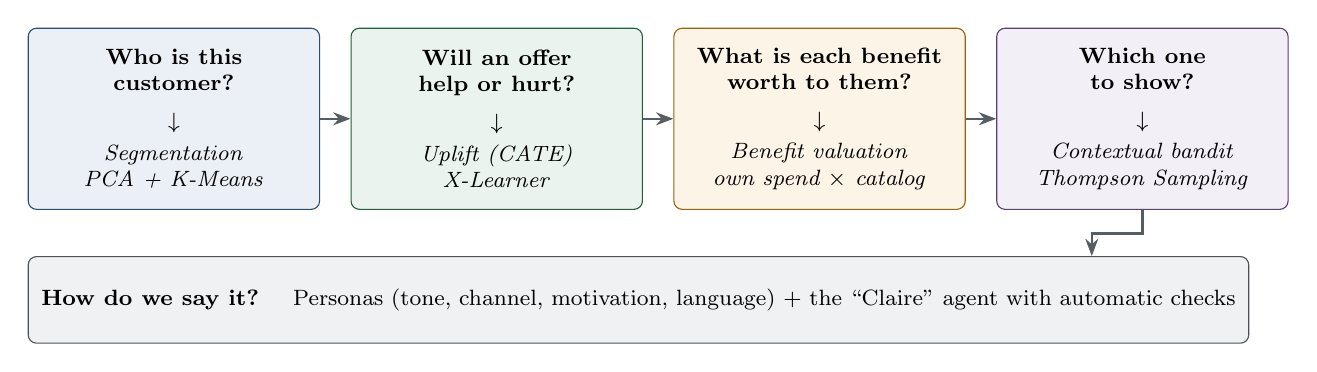
\begin{tikzpicture}[node distance=0pt]
\tikzset{qb/.style={draw=#1!70!black,fill=#1!10,rounded corners=3pt,minimum width=3.7cm,minimum height=2.3cm,align=center,font=\footnotesize,anchor=north west}}
\node[qb=cb] (q0) at (0,0) {\textbf{Who is this}\\\textbf{customer?}\\[4pt]$\downarrow$\\[2pt]\emph{Segmentation}\\\emph{PCA + K-Means}};
\node[qb=ct] (q1) at (4.1,0) {\textbf{Will an offer}\\\textbf{help or hurt?}\\[4pt]$\downarrow$\\[2pt]\emph{Uplift (CATE)}\\\emph{X-Learner}};
\node[qb=ca] (q2) at (8.2,0) {\textbf{What is each benefit}\\\textbf{worth to them?}\\[4pt]$\downarrow$\\[2pt]\emph{Benefit valuation}\\\emph{own spend $\times$ catalog}};
\node[qb=cp] (q3) at (12.3,0) {\textbf{Which one}\\\textbf{to show?}\\[4pt]$\downarrow$\\[2pt]\emph{Contextual bandit}\\\emph{Thompson Sampling}};
\foreach \i/\j in {0/1,1/2,2/3}{\draw[flow] (q\i.east) -- (q\j.west);}
\node[draw=cg!70!black,fill=cg!10,rounded corners=3pt,minimum width=15.5cm,minimum height=1.1cm,
      align=center,font=\footnotesize,anchor=north west] (say) at (0,-2.9)
      {\textbf{How do we say it?} \quad Personas (tone, channel, motivation, language) $+$ the ``Claire'' agent with automatic checks};
\draw[flow] (q3.south) -- ++(0,-0.3) -| ([xshift=-2cm]say.north east);
\end{tikzpicture}
\caption{Four decisions, one communication step. Each box consumes the output of the previous one.}
\end{figure}

\begin{center}
\small
\begin{tabularx}{\linewidth}{@{}p{2.6cm}p{3.8cm}X@{}}
\toprule
\textbf{Decision} & \textbf{Method} & \textbf{Why not something simpler?}\\
\midrule
Who? & Standardise $\to$ PCA(4) $\to$ K-Means, $k$ by silhouette & Business rules on raw columns would not capture joint behaviour; one latent space gives coherent, nameable groups.\\
Help or hurt? & X-Learner on a randomised campaign & ``Likely to upgrade'' is not ``caused to upgrade''. Big spenders upgrade anyway (waste) and over-indebted customers can be put off (harm).\\
What is it worth? & Per-user euro value from own MCC spend & A ``3\,\% cash-back'' promise means nothing without \emph{this} customer's spend and the cap.\\
Which one? & Linear Thompson Sampling over sectors & Showing the highest-value benefit ignores acceptance probability; a bandit trades off value and acceptance and keeps exploring.\\
How to say it? & LLM + hard checks + LLM judge & Free text is risky in banking: wrong currency, invented figures, over-promises.\\
\bottomrule
\end{tabularx}
\end{center}

% =====================================================================
\section{Architecture and data lineage}
% =====================================================================

\begin{figure}[h]
\centering
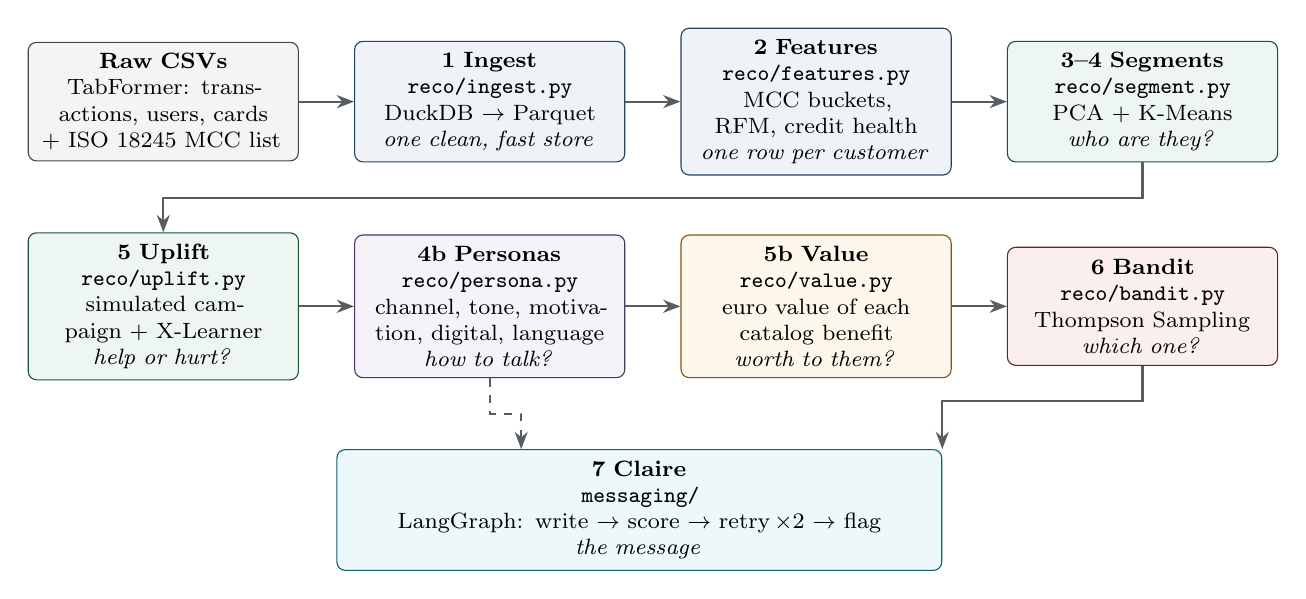
\begin{tikzpicture}[node distance=6mm and 7mm]
\node[stage=cg] (raw) {\textbf{Raw CSVs}\\TabFormer: transactions, users, cards\\+ ISO 18245 MCC list};
\node[stage=cb,right=of raw] (ing) {\textbf{1~Ingest}\\\code{reco/ingest.py}\\DuckDB $\to$ Parquet\\\emph{one clean, fast store}};
\node[stage=cb,right=of ing] (fea) {\textbf{2~Features}\\\code{reco/features.py}\\MCC buckets, RFM, credit health\\\emph{one row per customer}};
\node[stage=ct,right=of fea] (seg) {\textbf{3--4~Segments}\\\code{reco/segment.py}\\PCA + K-Means\\\emph{who are they?}};
\node[stage=ct,below=9mm of raw] (upl) {\textbf{5~Uplift}\\\code{reco/uplift.py}\\simulated campaign + X-Learner\\\emph{help or hurt?}};
\node[stage=cp,right=of upl] (per) {\textbf{4b~Personas}\\\code{reco/persona.py}\\channel, tone, motivation, digital, language\\\emph{how to talk?}};
\node[stage=ca,right=of per] (val) {\textbf{5b~Value}\\\code{reco/value.py}\\euro value of each catalog benefit\\\emph{worth to them?}};
\node[stage=cr,right=of val] (ban) {\textbf{6~Bandit}\\\code{reco/bandit.py}\\Thompson Sampling\\\emph{which one?}};
\node[stage=ck,below=9mm of per,xshift=1.9cm,text width=7.4cm] (cla) {\textbf{7~Claire}\\\code{messaging/}\\LangGraph: write $\to$ score $\to$ retry\,$\times$2 $\to$ flag\\\emph{the message}};
\draw[flow] (raw) -- (ing); \draw[flow] (ing) -- (fea); \draw[flow] (fea) -- (seg);
\draw[flow] (seg.south) -- ++(0,-4.5mm) -| (upl.north);
\draw[flow] (upl) -- (per);\draw[flow] (per) -- (val);\draw[flow] (val) -- (ban);
\draw[flow] (ban.south) -- ++(0,-4.5mm) -| (cla.north east);
\draw[dflow] (per.south) -- ++(0,-4.5mm) -| ([xshift=-1.5cm]cla.north);
\end{tikzpicture}
\caption{Pipeline overview. Solid arrows: main data flow. Dashed arrow: personas are consumed only by the last step.}
\label{fig:overview}
\end{figure}

\begin{center}
\small
\begin{tabularx}{\linewidth}{@{}p{5.7cm}p{1.9cm}X@{}}
\toprule
\textbf{Artifact} & \textbf{Produced by} & \textbf{Content}\\
\midrule
\code{warehouse/transactions/year=*} & ingest & 24.36\,M non-fraud transactions, partitioned by year\\
\texttt{warehouse/users, cards,}\texttt{ dim\_mcc} & ingest & demographics and credit, card types and limits, MCC dictionary\\
\code{warehouse/user_features} & features & 11 segmentation features $+$ 2 persona inputs per customer\\
\code{warehouse/user_mcc} & features & monthly spend, count and last-3-month spend per (customer, MCC, sector)\\
\code{segment.joblib} & segment & fitted scaler+PCA, K-Means\\
\code{user_scores} & uplift & features, cluster, simulated campaign, \code{cate}\\
\code{personas} & persona & five categorical traits $+$ languages\\
\code{user_benefit_value} & value & 18 benefits $\times$ 2\,000 customers: hard euro value, soft signal\\
\code{user_reco} & bandit & one offer per customer (sector, benefit, value, $p_{\text{accept}}$, upgrade gain)\\
\code{messages} & messaging & final text, attempts, full score grids as JSON\\
\bottomrule
\end{tabularx}
\end{center}

\why{Every stage writes a Parquet artifact. Stages can be re-run independently (the message step runs locally,
the heavy ingest ran on a CPU pod), and each artifact is inspectable and testable on its own.}

% =====================================================================
\section{Step 1 --- Ingest: CSV to a Parquet warehouse}
% =====================================================================

\textbf{What.} DuckDB reads the 2.3\,GB transaction CSV and writes it as Parquet, \emph{partitioned by year} and
sorted by customer and timestamp. Dollar strings become numbers, the timestamp is assembled from year/month/day/time,
and two flags are derived: \code{insufficient_balance} (from the error column) and \code{online}. Fraudulent
transactions are dropped. Users, cards and the ISO 18245 merchant-category (MCC) dictionary are written as small
tables.

\begin{figure}[h]
\centering
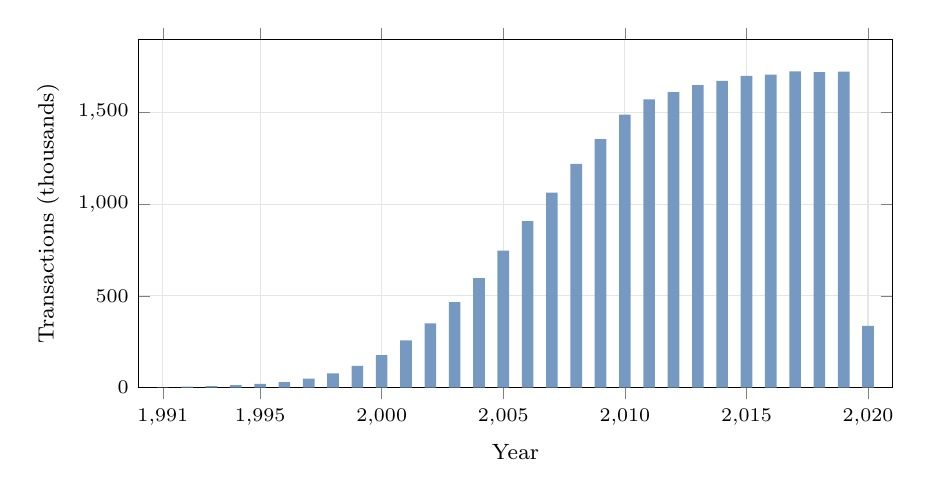
\begin{tikzpicture}
\begin{axis}[base,ybar,bar width=4.2pt,xlabel={Year},ylabel={Transactions (thousands)},
  xmin=1990,xmax=2021,ymin=0,xtick={1991,1995,2000,2005,2010,2015,2020},
  scaled y ticks=false,ytick distance=500]
\addplot[fill=cb!70,draw=none] coordinates {
(1991,1.6)(1992,5.1)(1993,8.4)(1994,14.3)(1995,20.9)(1996,29.9)(1997,49.7)(1998,78.3)(1999,118.2)
(2000,177.6)(2001,257.6)(2002,350.6)(2003,466.1)(2004,596.4)(2005,746.4)(2006,907.7)(2007,1062.6)
(2008,1219.8)(2009,1354.3)(2010,1487.4)(2011,1570.5)(2012,1609.5)(2013,1648.9)(2014,1671.3)
(2015,1698.1)(2016,1705.3)(2017,1723.1)(2018,1719.1)(2019,1721.9)(2020,336.5)};
\end{axis}
\end{tikzpicture}
\caption{Warehouse content: 24\,357\,143 transactions by year. Volume ramps up until about 2012 and then
plateaus; 2020 is truncated (data end on 28 Feb 2020). This shape matters for step~2: recency and ``last
30/90 days'' are measured against the dataset's own last timestamp, not today's date.}
\end{figure}

\why{
\begin{itemize}
\item \textbf{Parquet + DuckDB} turns an out-of-memory CSV into a columnar store that later steps query in seconds; it also runs on a modest CPU pod.
\item \textbf{Partition by year} keeps files a sane size. Partitioning by customer would create 2\,000+ tiny directories (a deliberate trade-off noted in the code).
\item \textbf{Fraud removed} because the offer decision should reflect legitimate behaviour; fraudulent spend would inflate spend and category shares.
\item \textbf{Cards table} is needed later: credit limit gives utilisation, card type separates credit from debit spend.
\end{itemize}}

% =====================================================================
\section{Step 2 --- Features: what each customer looks like}
% =====================================================================

\textbf{What.} Each transaction is joined to the MCC dictionary and tagged with a coarse \emph{bucket}
(travel, healthcare, cash advance, other; used for segmentation) and a fine \emph{sector} (14 sectors;
used for benefit matching). Per customer, the pipeline computes monthly RFM and credit-health features
(table below). It also writes a customer $\times$ MCC table of average monthly spend and count, which is the
input of benefit valuation in step~5b.

\begin{center}
\small
\begin{tabularx}{\linewidth}{@{}p{3.1cm}p{5.3cm}X@{}}
\toprule
\textbf{Feature} & \textbf{Definition} & \textbf{Why it is there}\\
\midrule
\code{recency_days} & days between last transaction and dataset end & dormancy; classic ``R'' of RFM\\
\code{freq_month} & mean transactions per active month & activity level; ``F''\\
\code{spend_month} & mean spend per active month & size of wallet; ``M''\\
\code{travel_share} & share of spend in travel MCCs (airlines, hotels, rental, \dots) & affinity for travel-centred premium benefits\\
\code{healthcare_share} & share in health MCCs & affinity for cover / security\\
\code{cash_advance_share} & share in ATM / cash MCCs & financial-stress signal\\
\code{travel_30d} & travel spend in the last 30 days & \emph{current} travel intent\\
\code{insufficient_rate} & share of transactions declined for balance & liquidity stress\\
\code{fico}, \code{dti} & credit score; debt / yearly income & creditworthiness, over-indebtedness\\
\code{utilization} & monthly credit-card spend / credit limit & revolving behaviour\\
\midrule
\code{online_share}, \code{age} & kept out of clustering & \emph{inputs to the personas only}, so segments are behavioural, not demographic\\
\bottomrule
\end{tabularx}
\end{center}

\begin{figure}[h]
\centering
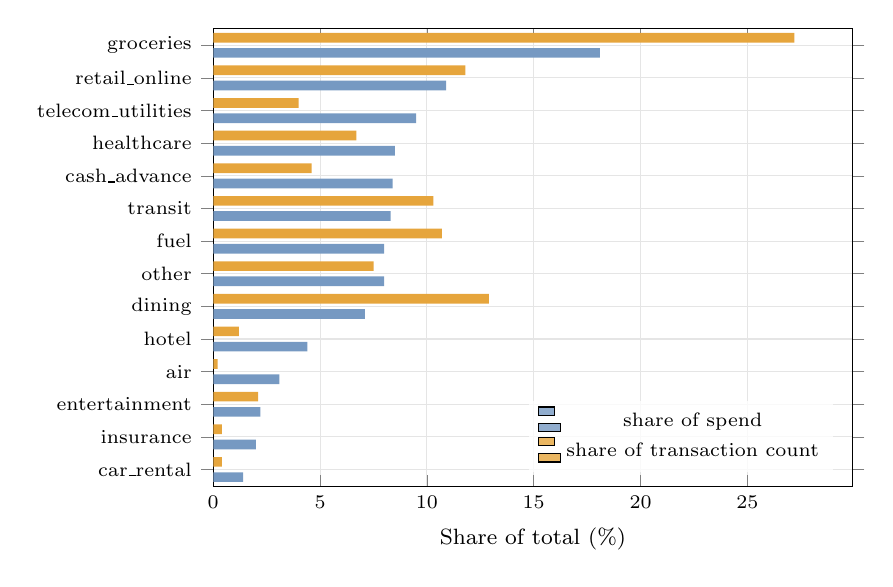
\begin{tikzpicture}
\begin{axis}[base,width=0.8\linewidth,height=7.4cm,xbar,bar width=3.5pt,xlabel={Share of total (\%)},
  symbolic y coords={groceries,retail\_online,telecom\_utilities,healthcare,cash\_advance,transit,fuel,other,dining,hotel,air,entertainment,insurance,car\_rental},
  ytick=data,y dir=reverse,xmin=0,legend pos=south east,enlarge y limits=0.04]
\addplot[fill=cb!70,draw=none] coordinates {(18.1,groceries)(10.9,retail\_online)(9.5,telecom\_utilities)(8.5,healthcare)(8.4,cash\_advance)(8.3,transit)(8.0,fuel)(8.0,other)(7.1,dining)(4.4,hotel)(3.1,air)(2.2,entertainment)(2.0,insurance)(1.4,car\_rental)};
\addplot[fill=ca!80,draw=none] coordinates {(27.2,groceries)(11.8,retail\_online)(4.0,telecom\_utilities)(6.7,healthcare)(4.6,cash\_advance)(10.3,transit)(10.7,fuel)(7.5,other)(12.9,dining)(1.2,hotel)(0.2,air)(2.1,entertainment)(0.4,insurance)(0.4,car\_rental)};
\legend{share of spend,share of transaction count}
\end{axis}
\end{tikzpicture}
\caption{Where the money goes versus where the swipes happen. Hotels and air are few swipes but big tickets
(4.4\,\% of spend from 1.2\,\% of transactions); groceries and dining are many small ones. This is why valuation
uses \emph{spend} for cash-back but \emph{counts} for the ``soft'' signal.}
\end{figure}

\begin{figure}[h]
\centering
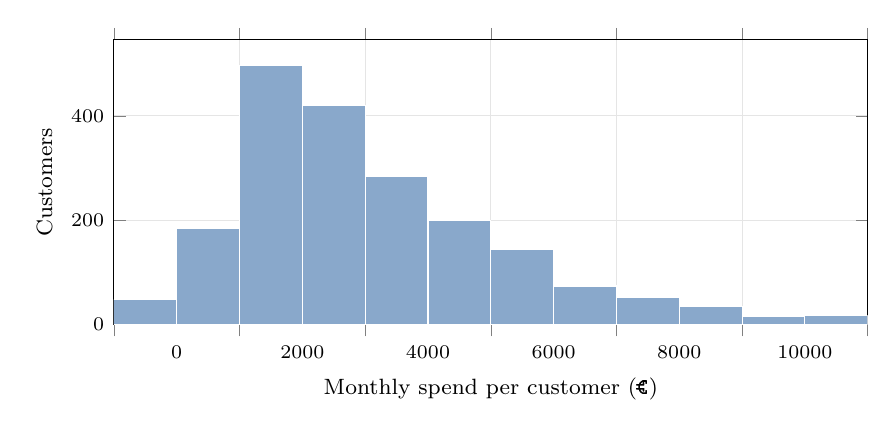
\begin{tikzpicture}
\begin{axis}[base,height=5.2cm,ybar interval,xlabel={Monthly spend per customer (\eur)},ylabel={Customers},
  xmin=0,xmax=12000,ymin=0,xtick={0,2000,...,12000},scaled x ticks=false,xticklabel style={/pgf/number format/1000 sep={}}]
\addplot[fill=cb!60,draw=white] coordinates {(0,48)(1000,184)(2000,496)(3000,419)(4000,283)(5000,199)(6000,145)(7000,74)(8000,52)(9000,34)(10000,15)(11000,17)(12000,0)};
\end{axis}
\end{tikzpicture}
\caption{Distribution of average monthly spend (values above \eur 12\,000 clipped into the last bin; maximum \eur 25\,223).
Median \eur 3\,631, mean \eur 4\,251: a long right tail of heavy spenders. This is why features are standardised before PCA
and why the uplift simulator uses $\log(1+\text{spend})$.}
\end{figure}

\why{
\begin{itemize}
\item \textbf{Deterministic SQL buckets, not a learned embedding}: auditable and explainable to a risk team (``travel = MCC 3000--3999 + 4511, 4722, 7011'').
\item \textbf{Monthly, not total, RFM}: customers differ in tenure; dividing by active months makes a 2-year and a 20-year customer comparable.
\item \textbf{Credit-health features} (FICO, DTI, utilisation, insufficient balance, cash advances) are what separate customers who should \emph{not} be sold a premium product.
\item \textbf{Excluding age/online share from clustering} prevents the segments from collapsing into demographics; personas can still use them later.
\end{itemize}}

% =====================================================================
\section{Steps 3--4 --- Segmentation: PCA and K-Means}
% =====================================================================

\textbf{What.} The 11 features are standardised, reduced to 4 principal components, and clustered with K-Means for
$k \in \{3,4,5,6\}$. The $k$ with the best silhouette score is kept, and each cluster is named by a transparent rule
(Figure~\ref{fig:naming}).

\begin{figure}[h]
\centering
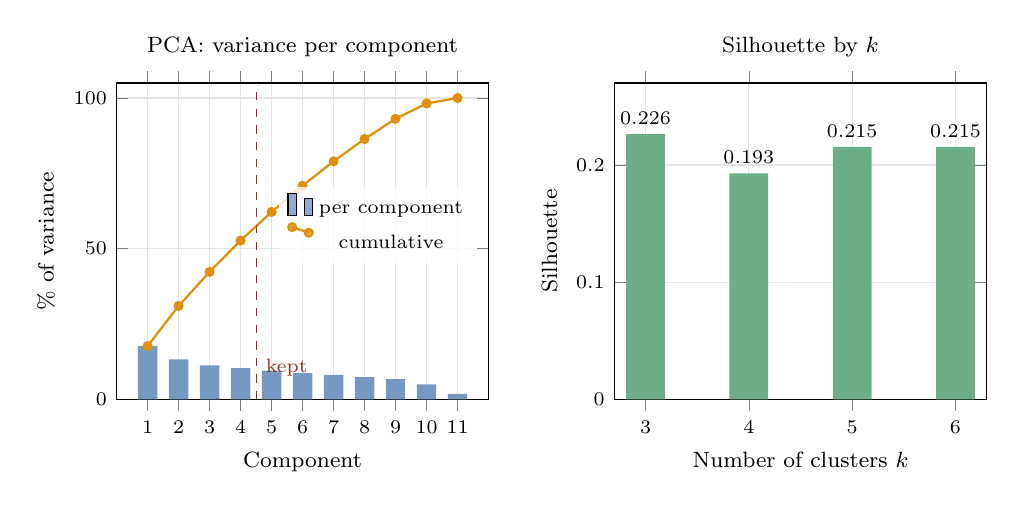
\begin{tikzpicture}
\begin{groupplot}[group style={group size=2 by 1,horizontal sep=1.6cm},width=0.52\linewidth,height=5.6cm]
\nextgroupplot[title={PCA: variance per component},ybar,bar width=7pt,xlabel={Component},ylabel={\% of variance},
  xtick={1,...,11},ymin=0,ymax=105,legend style={at={(0.97,0.55)},anchor=east}]
\addplot[fill=cb!70,draw=none] coordinates {(1,17.7)(2,13.3)(3,11.3)(4,10.4)(5,9.5)(6,8.7)(7,8.1)(8,7.4)(9,6.7)(10,5.0)(11,1.8)};
\addplot[sharp plot,thick,ca,mark=*,mark size=1.4pt,mark options={fill=ca}] coordinates {(1,17.7)(2,31.0)(3,42.3)(4,52.7)(5,62.2)(6,70.9)(7,79.0)(8,86.4)(9,93.1)(10,98.2)(11,100)};
\draw[dashed,cr!80!black] (axis cs:4.5,0) -- (axis cs:4.5,105) node[pos=0.1,right,font=\scriptsize,text=cr!80!black]{kept};
\legend{per component,cumulative}
\nextgroupplot[title={Silhouette by $k$},ybar,bar width=14pt,xlabel={Number of clusters $k$},ylabel={Silhouette},
  xtick={3,4,5,6},ymin=0,ymax=0.27,nodes near coords,every node near coord/.append style={font=\scriptsize},
  point meta=y,/pgf/number format/.cd,fixed,precision=3]
\addplot[fill=ct!70,draw=none] coordinates {(3,0.2264)(4,0.1929)(5,0.2154)(6,0.2154)};
\end{groupplot}
\end{tikzpicture}
\caption{Left: the 4 retained components capture 52.7\,\% of the variance; the rest is spread thinly, so the
space is denoised without discarding a dominant axis. Right: silhouette peaks at $k{=}3$ (0.226). $k{=}5,6$ are close
(0.215) but add segments the business could not act on differently.}
\end{figure}

\begin{center}
\small
\setlength{\tabcolsep}{4pt}
\newcommand{\hc}[1]{\pgfmathtruncatemacro{\ha}{min(80,abs(#1)*100)}\global\let\hag\ha\ifdim #1pt>0pt\cellcolor{cb!\hag}\else\cellcolor{cr!\hag}\fi #1}
\begin{tabular}{@{}lrrrr@{}}
\toprule
\textbf{Feature} & \textbf{PC1} & \textbf{PC2} & \textbf{PC3} & \textbf{PC4}\\
\midrule
recency\_days & \hc{-0.07} & \hc{-0.18} & \hc{-0.30} & \hc{-0.06}\\
freq\_month & \hc{0.64} & \hc{0.00} & \hc{-0.05} & \hc{-0.06}\\
spend\_month & \hc{0.65} & \hc{0.10} & \hc{-0.06} & \hc{-0.08}\\
travel\_share & \hc{-0.27} & \hc{0.59} & \hc{-0.05} & \hc{-0.15}\\
healthcare\_share & \hc{-0.03} & \hc{-0.43} & \hc{0.24} & \hc{-0.51}\\
cash\_advance\_share & \hc{0.14} & \hc{0.02} & \hc{-0.16} & \hc{0.70}\\
travel\_30d & \hc{0.12} & \hc{0.60} & \hc{-0.07} & \hc{-0.29}\\
insufficient\_rate & \hc{0.16} & \hc{-0.11} & \hc{0.39} & \hc{0.09}\\
fico & \hc{0.03} & \hc{0.14} & \hc{0.63} & \hc{0.03}\\
dti & \hc{-0.08} & \hc{-0.16} & \hc{-0.44} & \hc{-0.08}\\
utilization & \hc{0.15} & \hc{-0.06} & \hc{-0.25} & \hc{-0.35}\\
\bottomrule
\end{tabular}
\captionof{table}{PCA loadings (blue positive, red negative). PC1 = \emph{volume} (spend and frequency), PC2 = \emph{travel},
PC3 = \emph{credit quality} (FICO up; DTI, balance declines down), PC4 = \emph{cash-advance stress}. The components are interpretable,
which is what makes the clusters nameable.}
\end{center}

\begin{figure}[h]
\centering
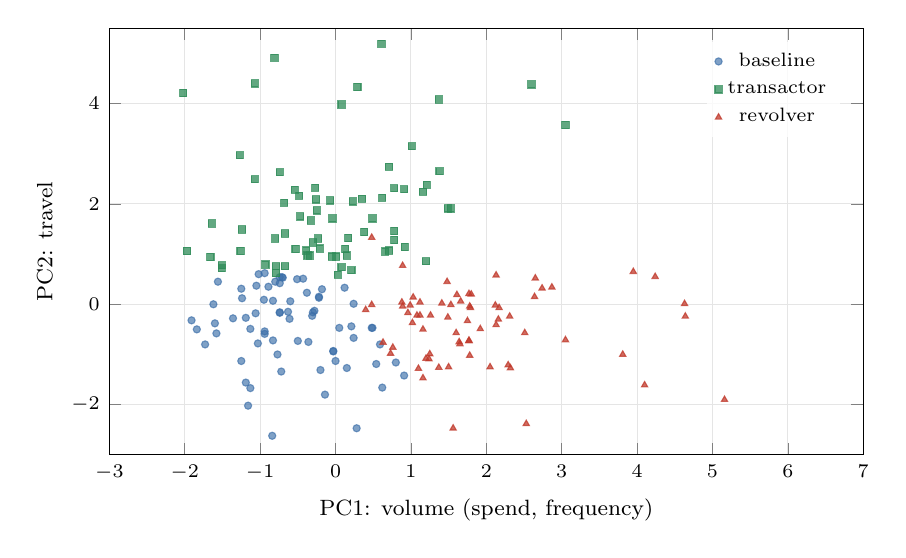
\begin{tikzpicture}
\begin{axis}[base,height=7cm,xlabel={PC1: volume (spend, frequency)},ylabel={PC2: travel},xmin=-3,xmax=7,ymin=-3,ymax=5.5,
  legend pos=north east,only marks,mark size=1.3pt]
\addplot[cb,mark=*,opacity=0.65] coordinates {(-0.28,-0.13)(-0.70,0.53)(-1.36,-0.28)(-0.30,-0.16)(-0.20,-1.31)(-0.95,0.09)(0.05,-0.47)(0.12,0.33)(0.24,-0.67)(-1.06,-0.18)(0.21,-0.44)(-0.03,-0.93)(0.00,-1.13)(-0.36,-0.75)(-0.77,-1.00)(0.48,-0.47)(-1.24,0.12)(-1.60,-0.38)(-1.13,-1.67)(-1.25,-1.13)(-1.16,-2.02)(-0.80,0.45)(-0.51,0.50)(0.80,-1.16)(-0.83,-0.72)(0.49,-0.47)(-0.94,-0.59)(0.24,0.01)(-0.74,0.42)(-1.03,-0.78)(-1.91,-0.32)(-0.43,0.51)(-0.18,0.30)(-0.74,-0.16)(-0.63,-0.15)(-0.71,0.54)(0.28,-2.47)(-1.84,-0.50)(-1.02,0.60)(-1.58,-0.58)(0.59,-0.80)(-1.73,-0.80)(0.54,-1.19)(-1.05,0.37)(-1.19,-1.56)(-1.19,-0.27)(-0.03,-0.94)(-0.61,-0.29)(-1.25,0.31)(-0.74,0.54)(-0.14,-1.80)(-0.38,0.23)(0.91,-1.42)(-0.74,-0.17)(-0.89,0.35)(-0.94,0.62)(-1.56,0.45)(0.15,-1.27)(-0.84,-2.62)(-1.13,-0.49)(-0.94,-0.54)(-0.22,0.13)(-0.22,0.15)(-0.50,-0.73)(-0.83,0.07)(-0.72,-1.34)(0.62,-1.66)(-1.62,0.00)(-0.31,-0.23)(-0.60,0.06)};
\addplot[ct,mark=square*,opacity=0.75] coordinates {(1.21,2.38)(-0.30,1.23)(-0.68,2.02)(0.17,1.32)(-0.93,0.79)(3.05,3.57)(0.03,0.59)(-0.39,1.07)(-1.97,1.06)(-0.79,0.62)(0.78,1.46)(0.01,0.95)(0.38,1.44)(-0.79,0.76)(-1.07,2.49)(0.61,5.19)(-1.26,1.06)(-0.80,1.31)(-1.51,0.72)(0.92,1.14)(-0.26,2.09)(-0.67,0.76)(-0.53,1.10)(-0.81,4.91)(0.13,1.10)(1.01,3.15)(0.08,3.98)(0.29,4.33)(-0.54,2.28)(-0.25,1.87)(-1.64,1.61)(-0.47,1.75)(-1.07,4.40)(-1.51,0.78)(0.21,0.68)(0.08,0.74)(0.71,2.74)(-0.67,1.41)(-0.37,0.97)(1.37,4.08)(0.78,2.31)(0.78,1.28)(-1.24,1.49)(-1.66,0.94)(-0.48,2.16)(-0.05,0.95)(0.35,2.10)(0.66,1.05)(1.20,0.86)(-0.04,1.71)(-0.33,1.67)(-0.34,0.97)(-1.27,2.97)(-0.21,1.11)(0.15,0.97)(0.23,2.05)(0.91,2.29)(0.49,1.71)(2.60,4.38)(1.49,1.91)(1.53,1.91)(0.71,1.07)(-0.23,1.31)(-0.07,2.07)(-2.02,4.21)(0.62,2.12)(1.16,2.24)(1.38,2.65)(-0.74,2.63)(-0.27,2.32)};
\addplot[cr,mark=triangle*,opacity=0.75] coordinates {(5.16,-1.90)(1.48,0.45)(1.03,0.14)(2.13,0.58)(1.08,-0.22)(0.73,-0.98)(1.77,0.21)(1.10,-1.28)(1.16,-0.50)(1.61,0.19)(0.96,-0.17)(2.12,-0.02)(1.79,-0.07)(3.95,0.65)(1.49,-0.26)(1.56,-2.47)(2.31,-0.24)(2.13,-0.41)(2.74,0.32)(1.66,0.06)(0.89,-0.04)(3.81,-1.00)(1.20,-1.08)(2.17,-0.07)(1.80,0.20)(1.75,-0.33)(0.89,0.77)(1.24,-1.09)(1.60,-0.57)(2.29,-1.21)(4.63,0.01)(2.32,-1.27)(1.77,-0.73)(1.26,-0.22)(2.51,-0.57)(1.12,0.04)(4.24,0.55)(2.87,0.34)(1.92,-0.49)(1.12,-0.22)(0.48,1.33)(1.77,-0.72)(2.16,-0.30)(0.48,-0.01)(1.65,-0.79)(4.64,-0.24)(1.50,-1.25)(1.64,-0.75)(2.53,-2.38)(1.78,-1.02)(1.41,0.02)(0.99,-0.02)(0.76,-0.86)(2.64,0.15)(1.78,-0.04)(4.10,-1.61)(0.88,0.04)(0.40,-0.11)(1.02,-0.37)(2.65,0.52)(0.63,-0.76)(1.37,-1.26)(2.05,-1.25)(3.05,-0.71)(1.16,-1.47)(1.25,-0.99)(1.53,-0.01)};
\legend{baseline,transactor,revolver}
\end{axis}
\end{tikzpicture}
\caption{The three segments in the first two principal components (70 random customers per segment; a few
extreme revolvers fall outside the window). Revolvers sit far right (high volume), transactors high on the travel axis,
the baseline group is the compact mass around the origin.}
\end{figure}

\begin{figure}[h]
\centering
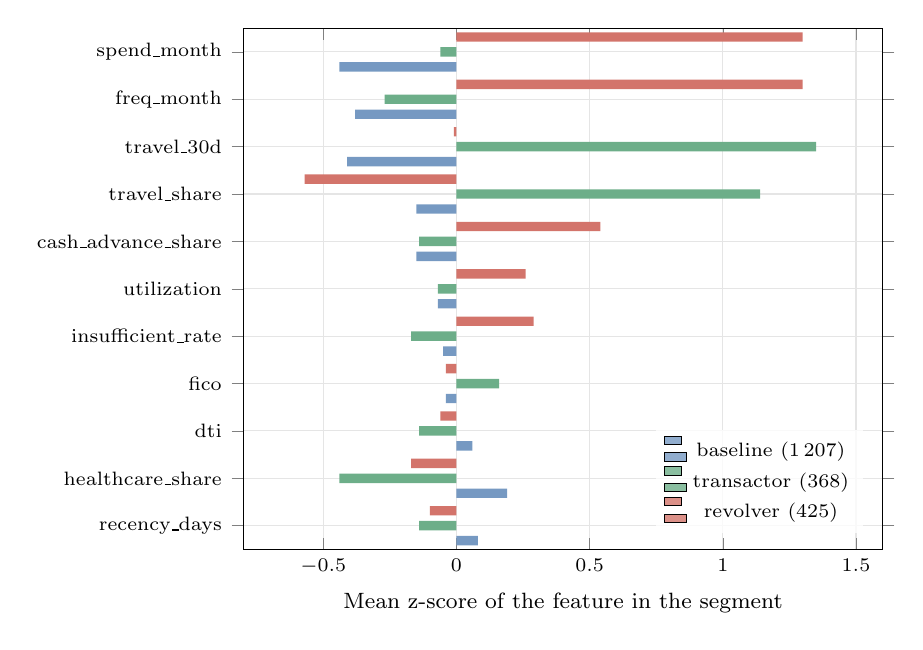
\begin{tikzpicture}
\begin{axis}[base,width=0.8\linewidth,height=8.2cm,xbar,bar width=3.4pt,xlabel={Mean z-score of the feature in the segment},
  symbolic y coords={spend\_month,freq\_month,travel\_30d,travel\_share,cash\_advance\_share,utilization,insufficient\_rate,fico,dti,healthcare\_share,recency\_days},
  ytick=data,y dir=reverse,enlarge y limits=0.05,legend pos=south east,xmin=-0.8,xmax=1.6]
\addplot[fill=cb!70,draw=none] coordinates {(-0.44,spend\_month)(-0.38,freq\_month)(-0.41,travel\_30d)(-0.15,travel\_share)(-0.15,cash\_advance\_share)(-0.07,utilization)(-0.05,insufficient\_rate)(-0.04,fico)(0.06,dti)(0.19,healthcare\_share)(0.08,recency\_days)};
\addplot[fill=ct!70,draw=none] coordinates {(-0.06,spend\_month)(-0.27,freq\_month)(1.35,travel\_30d)(1.14,travel\_share)(-0.14,cash\_advance\_share)(-0.07,utilization)(-0.17,insufficient\_rate)(0.16,fico)(-0.14,dti)(-0.44,healthcare\_share)(-0.14,recency\_days)};
\addplot[fill=cr!70,draw=none] coordinates {(1.30,spend\_month)(1.30,freq\_month)(-0.01,travel\_30d)(-0.57,travel\_share)(0.54,cash\_advance\_share)(0.26,utilization)(0.29,insufficient\_rate)(-0.04,fico)(-0.06,dti)(-0.17,healthcare\_share)(-0.10,recency\_days)};
\legend{baseline (1\,207),transactor (368),revolver (425)}
\end{axis}
\end{tikzpicture}
\caption{Segment profiles (z-scores against the whole population). \textbf{Transactors}: travel-heavy (+1.1 to +1.4~sd), good FICO,
low DTI. \textbf{Revolvers}: very high spend and frequency (+1.3~sd) \emph{and} the stress signals (cash advances +0.5, utilisation +0.3,
declines +0.3). \textbf{Baseline}: modest everything.}
\end{figure}

\begin{figure}[h]
\centering
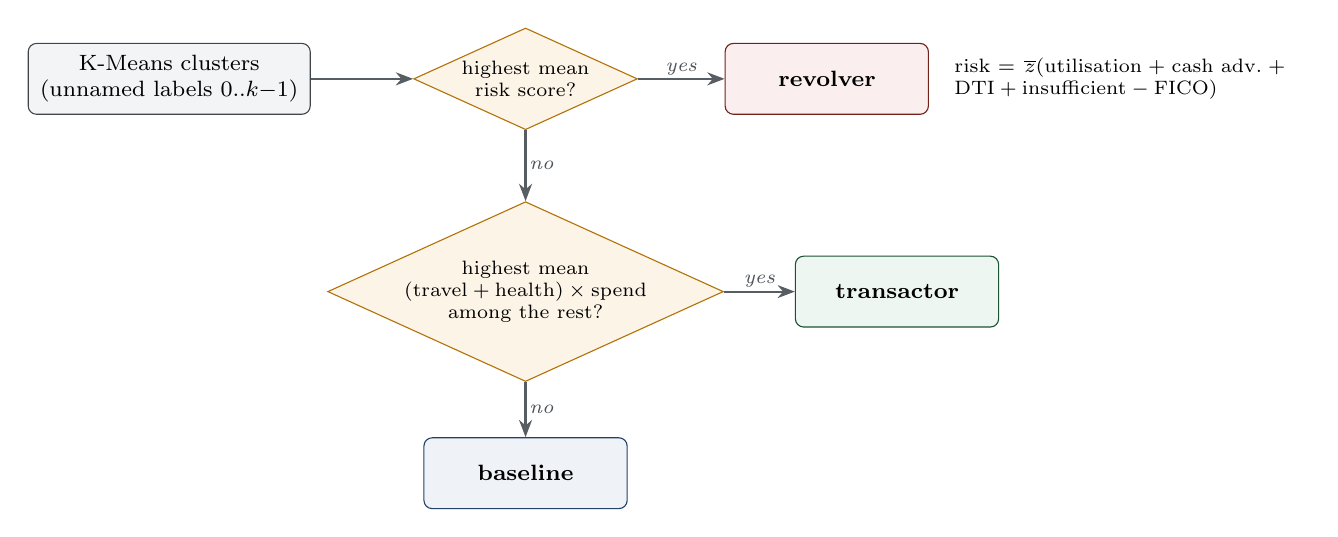
\begin{tikzpicture}[node distance=7mm]
\node[wide=cg,text width=3.3cm] (c) {K-Means clusters\\(unnamed labels 0..$k{-}1$)};
\node[dec,right=of c,xshift=6mm] (d1) {highest mean\\risk score?};
\node[wide=cr,right=of d1,xshift=4mm,text width=2.3cm] (rev) {\textbf{revolver}};
\node[dec,below=of d1,yshift=-2mm] (d2) {highest mean\\$(\text{travel}+\text{health})\times\text{spend}$\\among the rest?};
\node[wide=ct,right=of d2,xshift=2mm,text width=2.3cm] (tra) {\textbf{transactor}};
\node[wide=cb,below=of d2,text width=2.3cm] (bas) {\textbf{baseline}};
\draw[flow] (c)--(d1); \draw[flow] (d1)--node[above,lab]{yes}(rev);
\draw[flow] (d1)--node[right,lab]{no}(d2); \draw[flow] (d2)--node[above,lab]{yes}(tra);
\draw[flow] (d2)--node[right,lab]{no}(bas);
\node[right=2mm of rev,font=\scriptsize,align=left,text width=4.4cm]
  {risk $=\overline{z}(\text{utilisation}+\text{cash adv.}+\text{DTI}+\text{insufficient}-\text{FICO})$};
\end{tikzpicture}
\caption{Cluster naming. Labels from K-Means are arbitrary integers, so names are assigned by rules on cluster
centroids. This keeps the labelling reproducible across re-fits and the meaning auditable.}
\label{fig:naming}
\end{figure}

\why{
\begin{itemize}
\item \textbf{Scaling is mandatory}: spend is in thousands, shares are in $[0,1]$; unscaled K-Means would cluster on spend alone.
\item \textbf{PCA before K-Means} decorrelates the features (spend and frequency move together) and removes noise; distances in 4-D are more meaningful than in 11-D.
\item \textbf{Silhouette picks $k$}, instead of an arbitrary choice, and the search range 3--6 matches how many distinct treatments marketing can run.
\item \textbf{Named by rule}: ``revolver'' matters downstream (offers are suppressed), so the name must be derived from risk indicators, not from a human squinting at a plot.
\end{itemize}}

% =====================================================================
\section{Step 5 --- Uplift: should we even make the offer?}
% =====================================================================

\subsection{The idea}

Predicting who will upgrade is not enough. Four kinds of customer exist, and only one is worth contacting:

\begin{figure}[h]
\centering
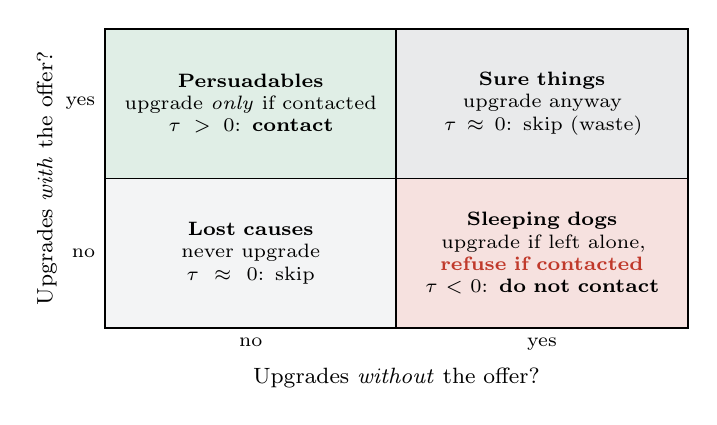
\begin{tikzpicture}[x=3.7cm,y=1.9cm]
\fill[ct!15] (0,1) rectangle (1,2); \fill[cg!15] (1,1) rectangle (2,2);
\fill[cg!8] (0,0) rectangle (1,1); \fill[cr!15] (1,0) rectangle (2,1);
\draw[thick] (0,0) rectangle (2,2); \draw[thick] (1,0)--(1,2); \draw (0,1)--(2,1);
\node[align=center,font=\scriptsize,text width=3.2cm] at (0.5,1.5) {\textbf{Persuadables}\\upgrade \emph{only} if contacted\\$\tau>0$: \textbf{contact}};
\node[align=center,font=\scriptsize,text width=3.2cm] at (1.5,1.5) {\textbf{Sure things}\\upgrade anyway\\$\tau\approx 0$: skip (waste)};
\node[align=center,font=\scriptsize,text width=3.2cm] at (0.5,0.5) {\textbf{Lost causes}\\never upgrade\\$\tau\approx 0$: skip};
\node[align=center,font=\scriptsize,text width=3.2cm] at (1.5,0.5) {\textbf{Sleeping dogs}\\upgrade if left alone,\\\textcolor{cr}{\textbf{refuse if contacted}}\\$\tau<0$: \textbf{do not contact}};
\node[below,font=\scriptsize] at (0.5,0) {no}; \node[below,font=\scriptsize] at (1.5,0) {yes};
\node[below=11pt,font=\footnotesize] at (1,0) {Upgrades \emph{without} the offer?};
\node[left,font=\scriptsize] at (0,1.5) {yes}; \node[left,font=\scriptsize] at (0,0.5) {no};
\node[rotate=90,font=\footnotesize] at (-0.2,1) {Upgrades \emph{with} the offer?};
\end{tikzpicture}
\caption{The uplift quadrants. Uplift modelling targets customers by $\tau(x)=\mathbb{E}[Y\mid T{=}1,x]-\mathbb{E}[Y\mid T{=}0,x]$,
the \emph{causal} gain from contacting them, rather than by their propensity to upgrade.}
\end{figure}

\subsection{Simulating the campaign}

The IBM data have no campaigns, so a randomised upgrade campaign is simulated with a known ground truth
(the code flags this as a deliberate stand-in for real campaign logs). With $\sigma$ the logistic function and
$s(\cdot)$ standardisation:
\begin{align*}
\text{affinity} &= s(\text{travel share}+\text{health share}),\\
\text{base} &= \sigma\!\big(-2.5 + 1.5\, s(\log(1+\text{spend}))\big),\\
\tau &= 0.3\,\sigma(2\,\text{affinity})\,(1-2\,\text{base}) \;-\; 0.15\cdot\mathbb{1}[\text{revolver}],\\
T &\sim \text{Bernoulli}(0.5), \qquad Y \sim \text{Bernoulli}\big(\text{clip}(\text{base}+T\,\tau,0,1)\big).
\end{align*}
Here base is the organic upgrade rate (big spenders upgrade anyway). The factor $(1-2\,\text{base})$ makes high-base customers (sure things) have low or negative uplift;
the $-0.15$ for revolvers encodes ``sleeping dogs''. Randomising $T$ at 50\,\% is what makes the estimated effect causal.

\subsection{The X-Learner}

\begin{figure}[h]
\centering
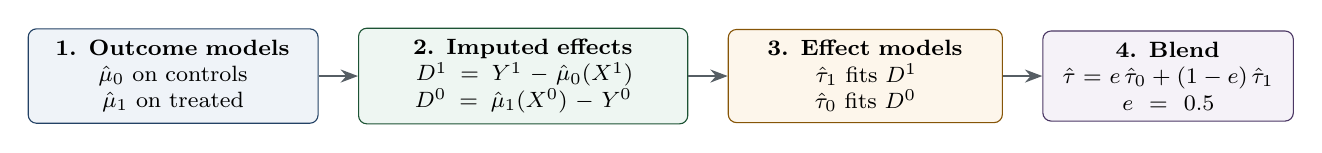
\begin{tikzpicture}[node distance=5mm]
\node[wide=cb,text width=3.4cm] (s1) {\textbf{1. Outcome models}\\$\hat\mu_0$ on controls\\$\hat\mu_1$ on treated};
\node[wide=ct,right=of s1,text width=3.9cm] (s2) {\textbf{2. Imputed effects}\\$D^1=Y^1-\hat\mu_0(X^1)$\\$D^0=\hat\mu_1(X^0)-Y^0$};
\node[wide=ca,right=of s2,text width=3.2cm] (s3) {\textbf{3. Effect models}\\$\hat\tau_1$ fits $D^1$\\$\hat\tau_0$ fits $D^0$};
\node[wide=cp,right=of s3,text width=2.9cm] (s4) {\textbf{4. Blend}\\$\hat\tau=e\,\hat\tau_0+(1-e)\,\hat\tau_1$\\$e=0.5$};
\draw[flow] (s1)--(s2); \draw[flow] (s2)--(s3); \draw[flow] (s3)--(s4);
\end{tikzpicture}
\caption{X-Learner. Each ``model'' is a depth-3 gradient-boosted regressor (\code{HistGradientBoostingRegressor}).
$e$ is the treatment probability (0.5 in a randomised trial).}
\end{figure}

\why{
\begin{itemize}
\item \textbf{X-Learner}: with unbalanced or modest sample sizes, each group's effect is learned from the \emph{other} group's imputed counterfactuals, so it generally beats a simple two-model difference; with a 50/50 split it is also easy to reason about.
\item \textbf{Features include the cluster dummy}, so segment-level heterogeneity (revolvers) can be learned.
\item \textbf{Shallow trees} (depth 3) regularise: with 2\,000 customers and a noisy 0/1 outcome, deeper trees would fit noise.
\end{itemize}}

\subsection{Did it work? (against the simulator's ground truth)}

\begin{figure}[h]
\centering
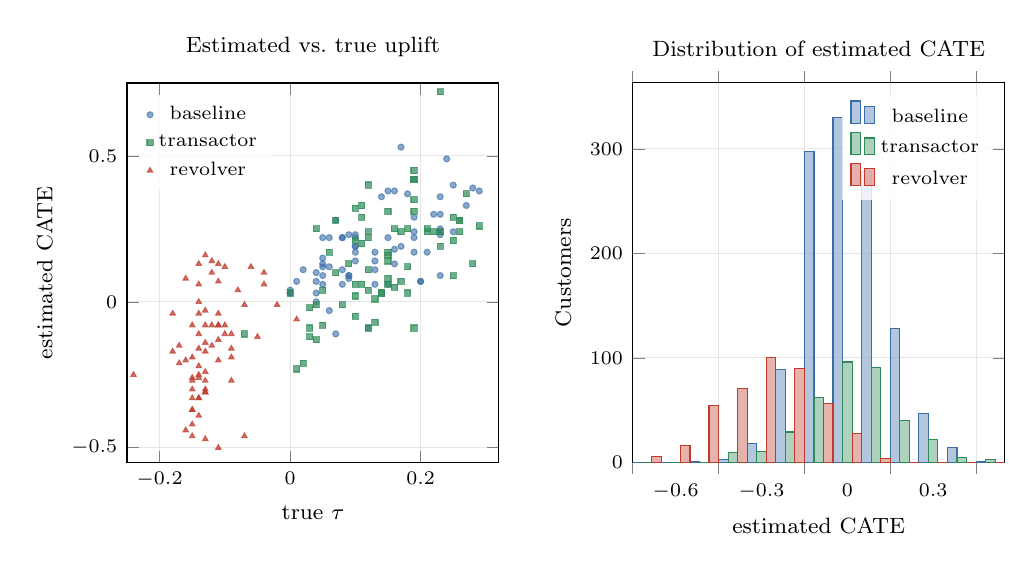
\begin{tikzpicture}
\begin{groupplot}[group style={group size=2 by 1,horizontal sep=1.7cm},width=0.52\linewidth,height=6.4cm]
\nextgroupplot[title={Estimated vs.\ true uplift},xlabel={true $\tau$},ylabel={estimated CATE},only marks,mark size=1.1pt,
  xmin=-0.25,xmax=0.32,ymin=-0.55,ymax=0.75,legend style={at={(0.03,0.97)},anchor=north west}]
\addplot[cb,mark=*,opacity=0.6] coordinates {(0.05,0.13)(0.14,0.36)(0.09,0.09)(0.15,0.22)(0.10,0.19)(0.25,0.24)(0.04,0.03)(0.10,0.14)(0.05,0.15)(0.15,0.06)(0.06,0.12)(0.10,0.19)(0.08,0.11)(0.16,0.38)(0.19,0.24)(0.00,0.03)(0.13,0.14)(0.27,0.33)(0.05,0.22)(0.23,0.23)(0.10,0.22)(0.19,0.22)(0.19,0.29)(0.13,0.06)(0.13,0.17)(0.15,0.38)(0.20,0.07)(0.07,-0.11)(0.23,0.09)(0.24,0.49)(0.29,0.38)(0.18,0.37)(0.05,0.09)(0.10,0.23)(0.08,0.06)(0.17,0.53)(0.04,0.10)(0.28,0.39)(0.23,0.30)(0.00,0.03)(0.07,0.28)(0.00,0.04)(0.01,0.07)(0.19,0.17)(0.02,0.11)(0.22,0.30)(0.08,0.22)(0.16,0.18)(0.06,-0.03)(0.13,0.11)(0.17,0.19)(0.09,0.08)(0.08,0.22)(0.10,0.17)(0.23,0.24)(0.21,0.17)(0.09,0.09)(0.23,0.25)(0.20,0.07)(0.25,0.40)(0.05,0.06)(0.09,0.23)(0.06,0.22)(0.04,-0.00)(0.16,0.13)(0.12,-0.09)(0.23,0.36)(0.04,0.07)(0.05,0.12)};
\addplot[ct,mark=square*,opacity=0.7] coordinates {(0.01,-0.23)(0.19,0.35)(0.21,0.24)(0.11,0.29)(0.15,0.31)(0.00,0.03)(0.10,0.32)(0.04,-0.01)(0.29,0.26)(0.19,0.31)(0.02,-0.21)(0.15,0.17)(0.03,-0.09)(0.12,0.22)(0.25,0.09)(0.12,-0.09)(0.23,0.24)(0.26,0.24)(0.25,0.29)(0.03,-0.02)(0.15,0.16)(0.08,-0.01)(0.18,0.12)(0.17,0.24)(0.21,0.25)(0.06,0.17)(0.10,0.02)(0.18,0.03)(0.15,0.08)(0.23,0.72)(0.27,0.37)(0.19,0.42)(0.25,0.21)(0.15,0.06)(0.04,0.25)(0.12,0.04)(0.10,-0.05)(0.16,0.05)(0.14,0.03)(0.07,0.28)(0.12,0.40)(0.05,-0.08)(0.23,0.19)(0.26,0.28)(0.22,0.24)(0.19,0.42)(0.13,0.01)(0.10,0.06)(0.10,0.21)(0.16,0.25)(0.13,-0.07)(0.11,0.06)(0.26,0.28)(0.15,0.14)(0.12,0.24)(0.11,0.20)(0.05,0.04)(0.19,0.45)(-0.07,-0.11)(0.03,-0.12)(0.04,-0.13)(0.07,0.10)(0.14,0.03)(0.17,0.07)(0.28,0.13)(0.09,0.13)(0.12,0.11)(0.11,0.33)(0.18,0.25)(0.19,-0.09)};
\addplot[cr,mark=triangle*,opacity=0.7] coordinates {(-0.14,-0.00)(-0.11,-0.08)(-0.14,-0.04)(-0.11,-0.20)(-0.14,-0.11)(-0.15,-0.08)(-0.13,-0.47)(-0.13,-0.14)(-0.14,-0.33)(-0.12,0.14)(-0.15,-0.19)(-0.13,-0.31)(-0.12,-0.15)(-0.16,0.08)(-0.11,-0.04)(-0.07,-0.46)(-0.15,-0.46)(-0.14,-0.39)(-0.16,-0.20)(-0.14,-0.22)(-0.13,-0.17)(-0.18,-0.04)(-0.04,0.06)(-0.15,-0.30)(-0.14,-0.26)(-0.09,-0.11)(-0.13,-0.24)(-0.12,-0.08)(-0.10,-0.08)(-0.07,-0.01)(-0.15,-0.42)(-0.12,0.10)(-0.13,-0.08)(-0.05,-0.12)(-0.15,-0.37)(-0.11,0.07)(-0.15,-0.26)(-0.18,-0.17)(-0.16,-0.44)(-0.11,-0.13)(-0.13,-0.27)(-0.26,0.01)(-0.10,-0.11)(-0.11,-0.08)(-0.14,-0.16)(-0.06,0.12)(-0.09,-0.16)(-0.17,-0.15)(-0.02,-0.01)(-0.11,-0.50)(-0.14,-0.33)(-0.08,0.04)(-0.13,-0.31)(-0.13,-0.03)(-0.11,0.13)(-0.13,-0.30)(-0.14,0.13)(-0.24,-0.25)(-0.04,0.10)(-0.10,0.12)(-0.14,0.06)(-0.15,-0.33)(-0.13,0.16)(-0.15,-0.37)(-0.09,-0.27)(-0.17,-0.21)(-0.15,-0.27)(-0.09,-0.19)(0.01,-0.06)(-0.14,-0.25)};
\addplot[no markers,black,dashed,forget plot] coordinates {(-0.25,-0.25)(0.32,0.32)};
\legend{baseline,transactor,revolver}
\nextgroupplot[title={Distribution of estimated CATE},ybar interval,xlabel={estimated CATE},ylabel={Customers},
  xmin=-0.6,xmax=0.7,ymin=0,xtick={-0.6,-0.3,0,0.3,0.6},legend style={at={(0.97,0.97)},anchor=north east}]
\addplot[fill=cb!60,fill opacity=0.65,draw=cb] coordinates {(-0.6,0)(-0.5,0)(-0.4,1)(-0.3,3)(-0.2,18)(-0.1,89)(0.0,297)(0.1,330)(0.2,278)(0.3,128)(0.4,47)(0.5,14)(0.6,1)(0.7,0)};
\addplot[fill=ct!60,fill opacity=0.65,draw=ct] coordinates {(-0.6,0)(-0.5,0)(-0.4,0)(-0.3,9)(-0.2,10)(-0.1,29)(0.0,62)(0.1,96)(0.2,91)(0.3,40)(0.4,22)(0.5,5)(0.6,3)(0.7,0)};
\addplot[fill=cr!60,fill opacity=0.65,draw=cr] coordinates {(-0.6,6)(-0.5,16)(-0.4,54)(-0.3,71)(-0.2,100)(-0.1,90)(0.0,56)(0.1,28)(0.2,4)(0.3,0)(0.4,0)(0.5,0)(0.6,0)(0.7,0)};
\legend{baseline,transactor,revolver}
\end{groupplot}
\end{tikzpicture}
\caption{Left: 70 customers per segment, estimated vs.\ true uplift (dashed = perfect). The estimates are noisy
(overall correlation 0.75) but ordered correctly, and the revolver cloud is clearly negative on both axes. Right:
the CATE distribution by segment. Revolvers centre near $-0.14$ (true mean $-0.125$); baseline and transactor centre near $+0.17$ (true $+0.13$ and $+0.17$).}
\end{figure}

\begin{figure}[h]
\centering
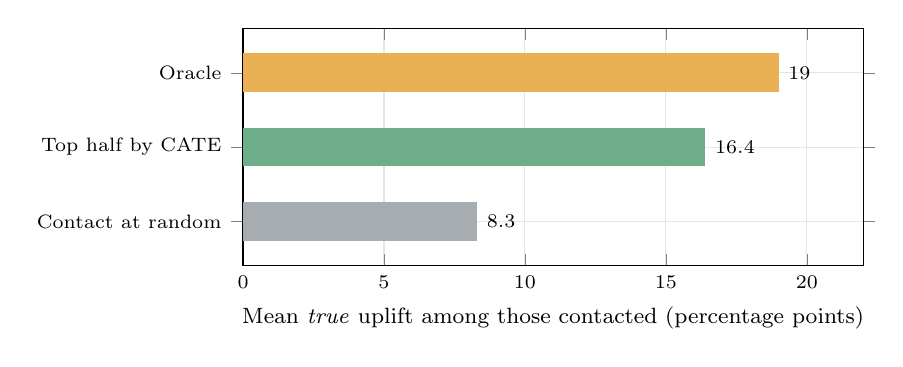
\begin{tikzpicture}
\begin{axis}[width=0.78\linewidth,height=4.6cm,xbar,bar width=14pt,xlabel={Mean \emph{true} uplift among those contacted (percentage points)},
  symbolic y coords={Oracle,Top half by CATE,Contact at random},
  ytick={Oracle,Top half by CATE,Contact at random},y dir=reverse,xmin=0,xmax=22,nodes near coords,every node near coord/.append style={font=\scriptsize},enlarge y limits=0.3]
\addplot[fill=cg!60,draw=none,bar shift=0pt] coordinates {(8.3,Contact at random)};
\addplot[fill=ct!70,draw=none,bar shift=0pt] coordinates {(16.4,Top half by CATE)};
\addplot[fill=ca!70,draw=none,bar shift=0pt] coordinates {(19.0,Oracle)};
\end{axis}
\end{tikzpicture}
\caption{Value of uplift targeting. Contacting the 1\,000 customers with the highest estimated CATE doubles the average
causal gain (8.3 $\to$ 16.4 points) and gets 86\,\% of the way to a perfect oracle (19.0). Caveat: evaluated on the
same customers the model was fit on, against a simulator I wrote; a held-out Qini curve on real logs is the real test.}
\end{figure}

\why{The uplift model does two jobs downstream: (i) its estimate is a feature of the bandit's context vector, and
(ii) it confirms that the ``revolver'' segment is a sleeping-dog population, 88 of whose 425 members nonetheless
get a slightly positive noisy estimate, which is exactly why suppression is done by a hard \emph{segment} rule rather
than trusting the per-customer estimate.}

% =====================================================================
\section{Step 4b --- Synthetic contact personas}
% =====================================================================

\textbf{What.} The bank has no contact-preference data, so each customer is assigned five seeded categorical traits
(digital level, channel, motivation, tone, languages). The draws are not uniform: their odds shift with observed behaviour via
multinomial logits (softmax of weighted inputs), and traits are drawn \emph{in order}, so later traits can depend on earlier ones.

\begin{figure}[h]
\centering
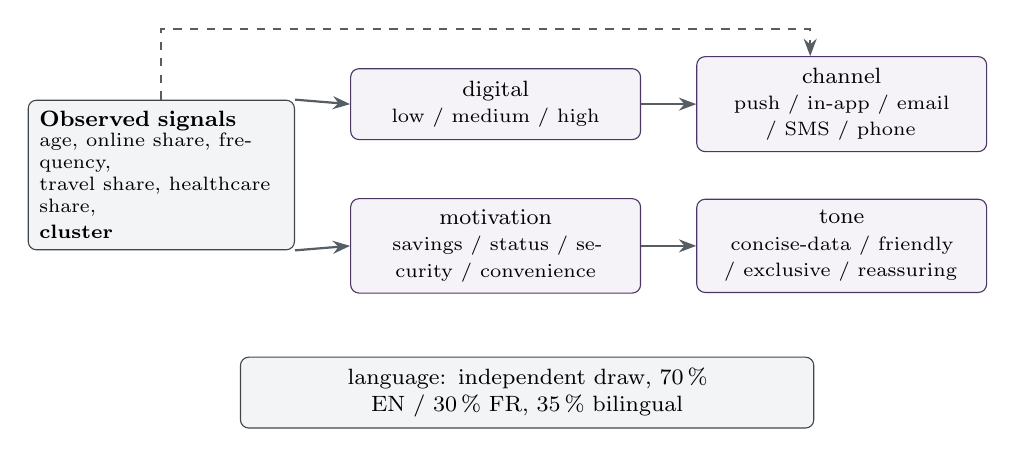
\begin{tikzpicture}[node distance=8mm and 7mm]
\node[wide=cg,text width=3.1cm,align=left] (sig) {\textbf{Observed signals}\\[-1pt]\scriptsize age, online share, frequency,\\\scriptsize travel share, healthcare share,\\\scriptsize \textbf{cluster}};
\node[wide=cp,right=of sig,yshift=9mm,text width=3.4cm] (dig) {digital\\\scriptsize low / medium / high};
\node[wide=cp,right=of sig,yshift=-9mm,text width=3.4cm] (mot) {motivation\\\scriptsize savings / status / security / convenience};
\node[wide=cp,right=of dig,text width=3.4cm] (cha) {channel\\\scriptsize push / in-app / email / SMS / phone};
\node[wide=cp,right=of mot,text width=3.4cm] (ton) {tone\\\scriptsize concise-data / friendly / exclusive / reassuring};
\node[wide=cg,below=of mot,xshift=4mm,text width=7cm] (lan) {language: independent draw, 70\,\% EN / 30\,\% FR, 35\,\% bilingual};
\draw[flow] (sig.north east) -- (dig.west); \draw[flow] (sig.south east) -- (mot.west);
\draw[flow] (dig)--(cha); \draw[flow] (mot)--(ton);
\draw[dflow] (sig.north) |- ([yshift=5mm]dig.north) -| ([xshift=-4mm]cha.north);
\end{tikzpicture}
\caption{Sampling graph. Dashed arrow: age also shifts the channel (older customers lean towards the phone).
Digital level drives the channel; motivation drives the tone.}
\end{figure}

\begin{center}
\small
\begin{tabularx}{\linewidth}{@{}p{2.1cm}X@{}}
\toprule
\textbf{Trait} & \textbf{Logit drivers (selection)}\\
\midrule
digital & high $\leftarrow$ online share $(+1.5)$, younger age, frequency; low $\leftarrow$ older age, low online share\\
channel & push/in-app $\leftarrow$ digital=high; SMS/phone $\leftarrow$ digital=low; phone also $\leftarrow$ age; email has a small bias\\
motivation & savings $\leftarrow$ revolver $(+1.5)$, baseline $(+0.7)$; status $\leftarrow$ transactor $(+1.2)$, travel share; security $\leftarrow$ healthcare share, age; convenience $\leftarrow$ frequency, online share\\
tone & concise-data $\leftarrow$ savings; friendly $\leftarrow$ convenience; exclusive $\leftarrow$ status; reassuring $\leftarrow$ security\\
\bottomrule
\end{tabularx}
\end{center}

\begin{figure}[h]
\centering
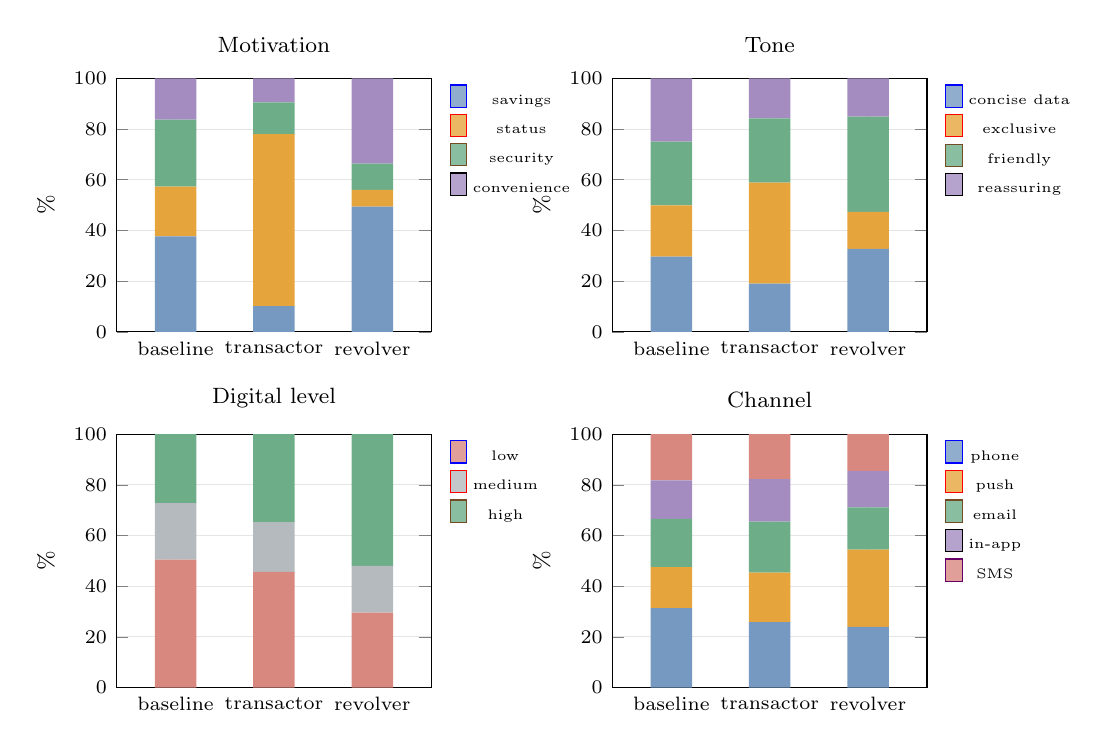
\begin{tikzpicture}
\pgfplotsset{persplot/.style={ybar stacked,bar width=15pt,symbolic x coords={baseline,transactor,revolver},xtick=data,ymin=0,ymax=100,enlarge x limits=0.3,
  ylabel={\%},legend style={font=\tiny,at={(1.03,1)},anchor=north west},width=0.46\linewidth,height=4.8cm}}
\begin{groupplot}[group style={group size=2 by 2,horizontal sep=2.3cm,vertical sep=1.3cm},persplot]
\nextgroupplot[title={Motivation}]
\addplot+[fill=cb!70,draw=none] coordinates {(baseline,37.7)(transactor,10.1)(revolver,49.4)};
\addplot+[fill=ca!80,draw=none] coordinates {(baseline,19.6)(transactor,67.9)(revolver,6.6)};
\addplot+[fill=ct!70,draw=none] coordinates {(baseline,26.4)(transactor,12.5)(revolver,10.4)};
\addplot+[fill=cp!70,draw=none] coordinates {(baseline,16.3)(transactor,9.5)(revolver,33.6)};
\legend{savings,status,security,convenience}
\nextgroupplot[title={Tone}]
\addplot+[fill=cb!70,draw=none] coordinates {(baseline,29.7)(transactor,19.0)(revolver,32.7)};
\addplot+[fill=ca!80,draw=none] coordinates {(baseline,20.2)(transactor,39.9)(revolver,14.6)};
\addplot+[fill=ct!70,draw=none] coordinates {(baseline,25.2)(transactor,25.3)(revolver,37.6)};
\addplot+[fill=cp!70,draw=none] coordinates {(baseline,24.9)(transactor,15.8)(revolver,15.1)};
\legend{concise data,exclusive,friendly,reassuring}
\nextgroupplot[title={Digital level}]
\addplot+[fill=cr!60,draw=none] coordinates {(baseline,50.5)(transactor,45.7)(revolver,29.6)};
\addplot+[fill=cg!50,draw=none] coordinates {(baseline,22.3)(transactor,19.6)(revolver,18.4)};
\addplot+[fill=ct!70,draw=none] coordinates {(baseline,27.3)(transactor,34.8)(revolver,52.0)};
\legend{low,medium,high}
\nextgroupplot[title={Channel}]
\addplot+[fill=cb!70,draw=none] coordinates {(baseline,31.4)(transactor,25.8)(revolver,24.0)};
\addplot+[fill=ca!80,draw=none] coordinates {(baseline,16.1)(transactor,19.6)(revolver,30.4)};
\addplot+[fill=ct!70,draw=none] coordinates {(baseline,19.1)(transactor,20.1)(revolver,16.7)};
\addplot+[fill=cp!70,draw=none] coordinates {(baseline,15.2)(transactor,16.8)(revolver,14.4)};
\addplot+[fill=cr!60,draw=none] coordinates {(baseline,18.2)(transactor,17.7)(revolver,14.6)};
\legend{phone,push,email,in-app,SMS}
\end{groupplot}
\end{tikzpicture}
\caption{Persona mix by segment (share of each segment, \%). The signals behave as designed: status dominates transactors (68\,\%),
savings dominates revolvers (49\,\%), and revolvers skew digital (52\,\% high) and push. The mix is intentionally \emph{soft}: no persona is deterministic.}
\end{figure}

\why{
\begin{itemize}
\item \textbf{Correlated, not uniform}: uniform random personas would make every downstream test trivially fine. Realistic correlations (digital $\to$ channel, status $\to$ exclusive tone) stress the message agent with coherent but varied inputs.
\item \textbf{Softmax with sequential dependence} gives a small, readable, tunable generative model.
\item \textbf{Seeded}: identical personas on every run, so results are reproducible and diff-able.
\end{itemize}}

\begin{warnbox}
\textbf{Honest label.} These personas are \emph{invented distributions conditioned on real signals}, not measured
preferences. Replace the weights with ones fitted on actual channel-engagement and response data once messages have been sent.
\end{warnbox}

% =====================================================================
\section{Step 5b --- Benefit valuation: what is each offer worth, in euros?}
% =====================================================================

\textbf{What.} A catalog of 18 benefits across two tiers is defined in \code{benefits.csv}. For each customer and each benefit, the pipeline
computes a monthly value from \emph{that customer's own spend per MCC}.

\begin{center}
\scriptsize
\setlength{\tabcolsep}{3pt}
\begin{tabular}{@{}llllr@{}}
\toprule
\textbf{Tier} & \textbf{Benefit} & \textbf{Kind} & \textbf{Sector} & \textbf{Rule}\\
\midrule
standard & cash-back, all purchases & cashback & all & 0.5\,\%, cap \eur 10/mo\\
standard & cash-back, groceries & cashback & groceries & 1\,\%, cap \eur 15/mo\\
standard & Air France / Hilton points & partner points & air / hotel & 1\,\% of partner MCC spend\\
standard & purchase insurance & insurance & retail online & cap \eur 5/mo (nominal \eur 3)\\
standard & streaming & subscription & entertainment & price \eur 8/mo (nominal \eur 4)\\
\midrule
premium & cash-back, all purchases & cashback & all & 1\,\%, cap \eur 20/mo\\
premium & cash-back dining / fuel / hotel & cashback & dining / fuel / hotel & 3\,\% (cap \eur 30/15) / 5\,\% (cap \eur 40)\\
premium & BA / Singapore / Hilton points & partner points & air / hotel & 3\,\% of partner MCC spend\\
premium & travel / car-rental insurance & insurance & air / car rental & cap \eur 25 / \eur 15 (nominal \eur 15 / 8)\\
premium & streaming, phone plan, gym & subscription & entertainment / telecom & price \eur 12 / 20 / 30 (nominal \eur 6 / 10 / 12)\\
\midrule
\multicolumn{5}{@{}l}{\textbf{Premium annual fee: \eur 240 (\eur 20/month).}}\\
\bottomrule
\end{tabular}
\end{center}

\begin{figure}[h]
\centering
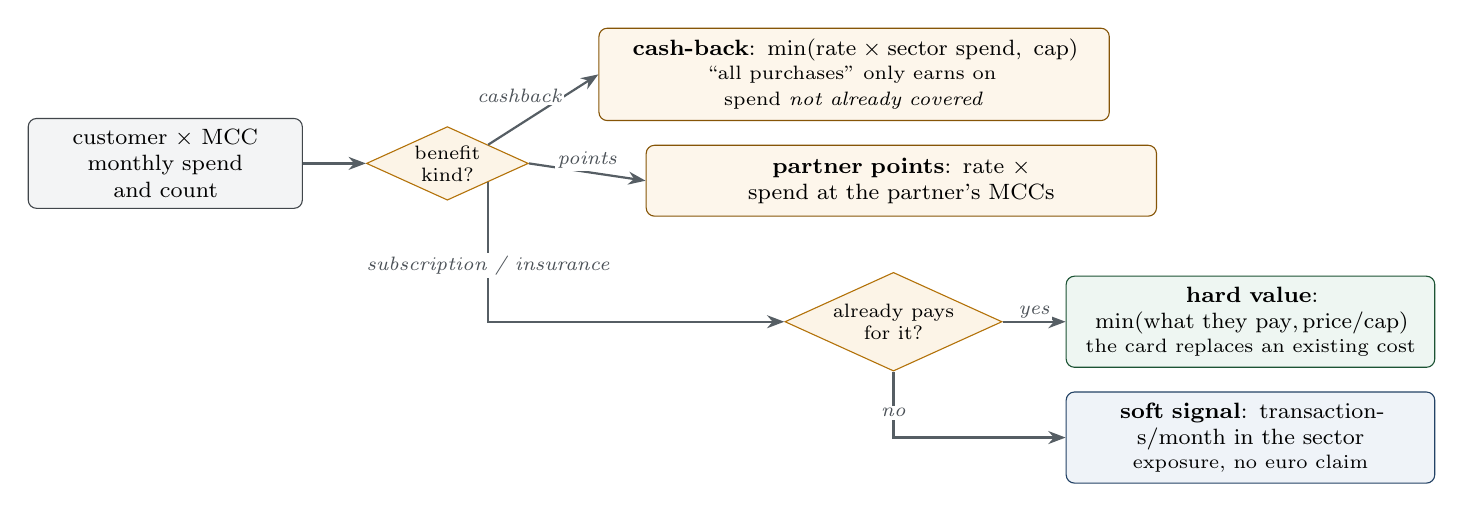
\begin{tikzpicture}[node distance=6mm and 8mm]
\node[wide=cg,text width=3.2cm] (u) {customer $\times$ MCC\\monthly spend and count};
\node[dec,right=of u] (k) {benefit\\kind?};
\node[wide=ca,above right=3mm and 14mm of k,text width=6.2cm] (cb1) {\textbf{cash-back}: $\min(\text{rate}\times\text{sector spend},\ \text{cap})$\\[-1pt]\scriptsize ``all purchases'' only earns on spend \emph{not already covered}};
\node[wide=ca,right=of k,yshift=-0.2cm,xshift=6mm,text width=6.2cm,below=1mm of cb1] (pp) {\textbf{partner points}: rate $\times$ spend at the partner's MCCs};
\node[dec,below=7mm of pp,xshift=-1mm] (pay) {already pays\\for it?};
\node[wide=ct,right=8mm of pay,text width=4.4cm] (hard) {\textbf{hard value}: $\min(\text{what they pay},\text{price/cap})$\\[-1pt]\scriptsize the card replaces an existing cost};
\node[wide=cb,below=3mm of hard,text width=4.4cm] (soft) {\textbf{soft signal}: transactions/month in the sector\\[-1pt]\scriptsize exposure, no euro claim};
\draw[flow] (u)--(k); \draw[flow] (k.north east)--node[left,lab,pos=0.7]{cashback}(cb1.west);
\draw[flow] (k.east)--node[above,lab]{points}(pp.west);
\draw[flow] (k.south east) |- node[below,lab,pos=0.25]{subscription / insurance}(pay.west);
\draw[flow] (pay)--node[above,lab]{yes}(hard); \draw[flow] (pay.south)|-node[below,lab,pos=0.25]{no}(soft.west);
\end{tikzpicture}
\caption{Valuation logic per benefit kind. The rule that \emph{only money the customer can be seen to spend counts as hard value}
keeps the numbers defendable.}
\end{figure}

\paragraph{Cash-back does not stack.} If a premium customer earns 3\,\% on dining, that dining spend should not
\emph{also} earn the 1\,\% ``all purchases'' rate. For tier $t$, let $c_s(\cdot)$ be the spend in sector $s$
that already earns a sector rate (up to its cap):
\[
\text{covered}_t=\sum_{s}\min\!\Big(\text{spend}_s,\ \tfrac{\text{cap}_s}{\text{rate}_s}\Big),\qquad
\text{value}^{\text{all}}_t=\min\big(\text{rate}_{\text{all}}\,(\text{total}-\text{covered}_t),\ \text{cap}_{\text{all}}\big).
\]
The monthly gain of upgrading, net of the fee, then compares the two tiers' totals:
\[
\text{upgrade\_gain}=\sum\text{tier value}_{\text{premium}}-\sum\text{tier value}_{\text{standard}}-\frac{240}{12}.
\]

\begin{figure}[h]
\centering
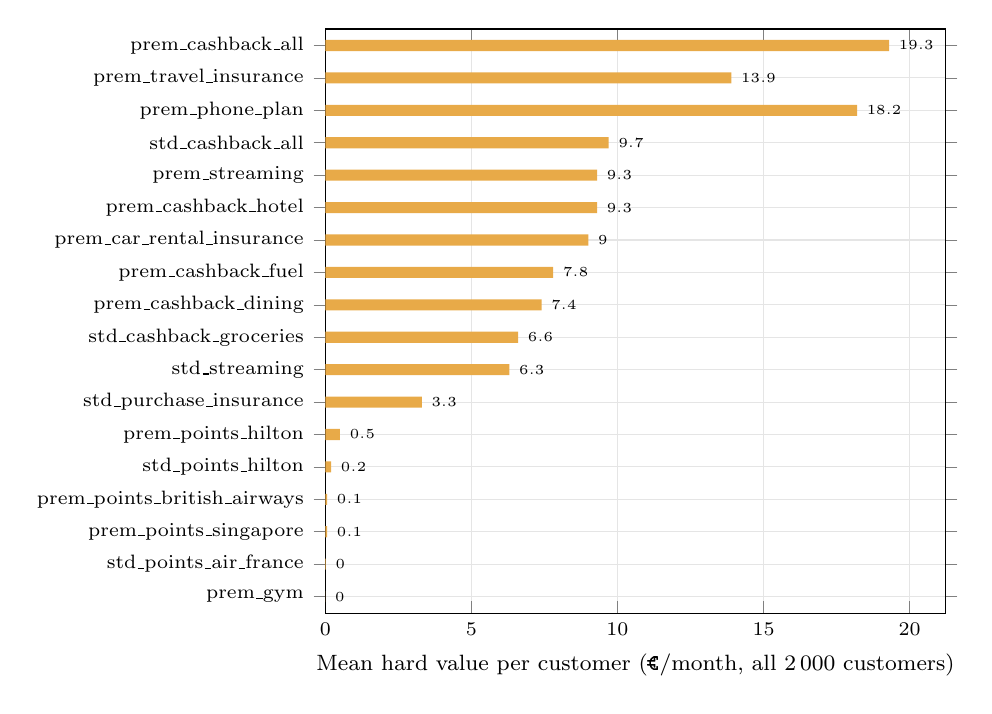
\begin{tikzpicture}
\begin{axis}[base,width=0.78\linewidth,height=9cm,xbar,bar width=4pt,xlabel={Mean hard value per customer (\eur/month, all 2\,000 customers)},
  symbolic y coords={prem\_cashback\_all,prem\_travel\_insurance,prem\_phone\_plan,std\_cashback\_all,prem\_streaming,prem\_cashback\_hotel,prem\_car\_rental\_insurance,prem\_cashback\_fuel,prem\_cashback\_dining,std\_cashback\_groceries,std\_streaming,std\_purchase\_insurance,prem\_points\_hilton,std\_points\_hilton,prem\_points\_british\_airways,prem\_points\_singapore,std\_points\_air\_france,prem\_gym},
  ytick=data,y dir=reverse,xmin=0,enlarge y limits=0.03,
  nodes near coords,every node near coord/.append style={font=\tiny},/pgf/number format/.cd,fixed,precision=1]
\addplot[fill=ca!75,draw=none] coordinates {(19.3,prem\_cashback\_all)(13.9,prem\_travel\_insurance)(18.2,prem\_phone\_plan)(9.7,std\_cashback\_all)(9.3,prem\_streaming)(9.3,prem\_cashback\_hotel)(9.0,prem\_car\_rental\_insurance)(7.8,prem\_cashback\_fuel)(7.4,prem\_cashback\_dining)(6.6,std\_cashback\_groceries)(6.3,std\_streaming)(3.3,std\_purchase\_insurance)(0.5,prem\_points\_hilton)(0.2,std\_points\_hilton)(0.06,prem\_points\_british\_airways)(0.06,prem\_points\_singapore)(0.02,std\_points\_air\_france)(0,prem\_gym)};
\end{axis}
\end{tikzpicture}
\caption{Average hard value of each benefit across the base. Cash-back on all purchases is worth the most on
average, mostly because \emph{every} customer earns it (100\,\% coverage) and it hits the \eur 20 cap. Partner points are worth
almost nothing because few customers spend at those specific airlines. The gym has zero hard value for everybody (no matching spend in the data) and only a soft signal ($95\,\%$ of customers have some transactions in the sector).}
\end{figure}

\begin{figure}[h]
\centering
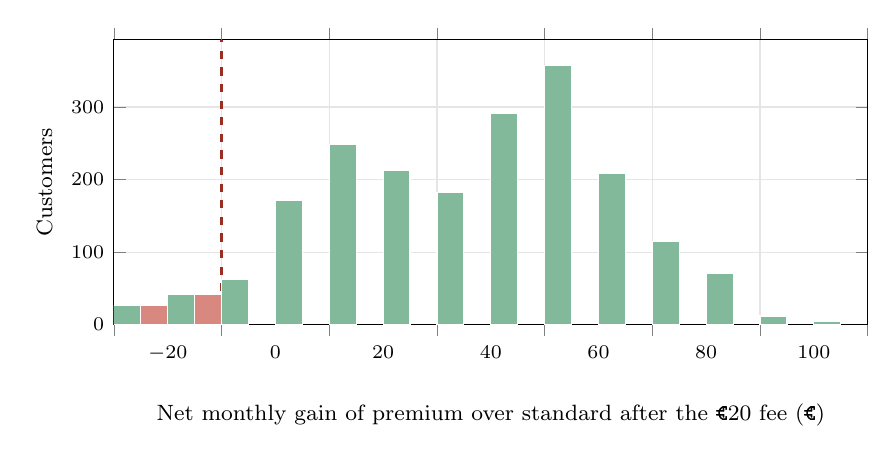
\begin{tikzpicture}
\begin{axis}[base,height=5.2cm,ybar interval,xlabel={Net monthly gain of premium over standard after the \eur 20 fee (\eur)},ylabel={Customers},
  xmin=-20,xmax=120,ymin=0,xtick={-20,0,...,120},extra x ticks={0},extra x tick style={grid=major,grid style={dashed,cr!80!black,thick}}]
\addplot[fill=ct!60,draw=white] coordinates {(-20,27)(-10,41)(0,62)(10,171)(20,248)(30,212)(40,182)(50,291)(60,357)(70,208)(80,115)(90,70)(100,12)(110,4)(120,0)};
\addplot[fill=cr!60,draw=white] coordinates {(-20,27)(-10,41)(0,0)};
\end{axis}
\end{tikzpicture}
\caption{Net gain of upgrading (all 2\,000 customers). 96.6\,\% of customers would gain from the premium card on their own spend; 68 customers (3.4\,\%) would lose money. Median $\approx$ \eur 53/month.}
\end{figure}

\why{
\begin{itemize}
\item \textbf{Own-spend valuation} makes ``\eur 20 a month'' a statement about \emph{this} customer, which is what lets the message be concrete and truthful.
\item \textbf{Non-stacking cash-back} avoids double counting, the most common way to oversell a card.
\item \textbf{Hard vs.\ soft} separates measurable money from speculative interest; the soft signal can still rank an offer, but it never becomes a euro claim in a message beyond a flagged nominal value.
\item \textbf{Net of fee} (\eur 240/year) is the honest bottom line for a premium upgrade.
\end{itemize}}

% =====================================================================
\section{Step 6 --- The bandit: choosing one offer per customer}
% =====================================================================

\subsection{Candidate generation}

\begin{figure}[h]
\centering
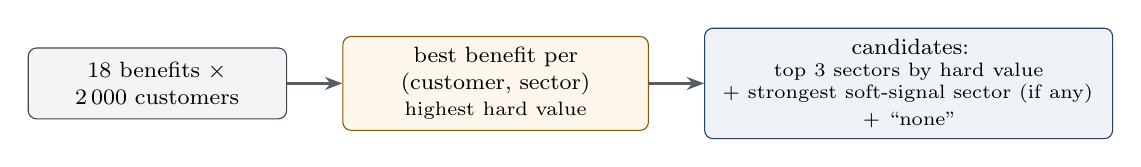
\begin{tikzpicture}[node distance=7mm]
\node[wide=cg,text width=3cm] (v) {18 benefits $\times$ 2\,000 customers};
\node[wide=ca,right=of v,text width=3.6cm] (b) {best benefit per (customer, sector)\\\scriptsize highest hard value};
\node[wide=cb,right=of b,text width=4.9cm] (c) {candidates:\\\scriptsize top 3 sectors by hard value\\\scriptsize $+$ strongest soft-signal sector (if any)\\\scriptsize $+$ ``none''};
\draw[flow] (v)--(b); \draw[flow] (b)--(c);
\end{tikzpicture}
\caption{Each customer ends up with 3 or 4 real candidates (mean 3.44) plus the option to do nothing. Restricting the choice to the top few keeps the bandit's job small and explainable.}
\end{figure}

\subsection{Linear Thompson Sampling}

There is one arm per sector: the 14 sectors plus ``all'' (generic cash-back) and ``none'' (do nothing), i.e. 16 arms.
Each arm $a$ keeps a Bayesian linear model $\theta_a$ over an 8-dimensional \textbf{context}
$x$: three segment one-hots, normalised log hard value, normalised log soft signal, the \textbf{CATE from step~5}, log of travel spend in the last 30 days, and a bias.
At each step:
\[
\tilde\theta_a\sim\mathcal{N}\!\big(A_a^{-1}b_a,\ v^2A_a^{-1}\big),\quad
a^\star=\arg\max_{a\in\text{candidates}}\, x_a^\top\tilde\theta_a,\quad
A_{a^\star}\mathrel{+}=x x^\top,\ \ b_{a^\star}\mathrel{+}=r\,x,\qquad v=0.3.
\]

\begin{figure}[h]
\centering
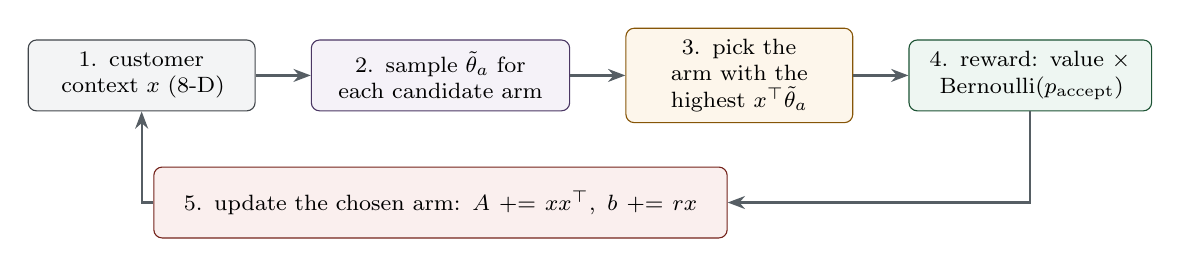
\begin{tikzpicture}[node distance=7mm]
\node[wide=cg,text width=2.6cm] (x) {1. customer context $x$ (8-D)};
\node[wide=cp,right=of x,text width=3cm] (s) {2. sample $\tilde\theta_a$ for each candidate arm};
\node[wide=ca,right=of s,text width=2.6cm] (a) {3. pick the arm with the highest $x^\top\tilde\theta_a$};
\node[wide=ct,right=of a,text width=2.8cm] (r) {4. reward: value $\times$ Bernoulli($p_{\text{accept}}$)};
\node[wide=cr,below=7mm of s,text width=7cm] (u) {5. update the chosen arm: $A\mathrel{+}=xx^\top,\ b\mathrel{+}=rx$};
\draw[flow] (x)--(s); \draw[flow] (s)--(a); \draw[flow] (a)--(r);
\draw[flow] (r.south) |- (u.east); \draw[flow] (u.west) -| (x.south);
\end{tikzpicture}
\caption{One bandit round. Exploration is built in: arms with little data have a wide posterior, so they occasionally win.}
\end{figure}

\subsection{The simulated environment}

No campaign logs exist, so acceptance is simulated:
\[
p_{\text{accept}}=\sigma\!\big(-2+1.5\,h+1.0\,s\cdot \rho_k+\text{affinity}_{k,\text{arm}}\big),\qquad
r=\text{value}\times\text{Bernoulli}(p_{\text{accept}}),
\]
where $h,s$ are the normalised hard and soft signals, $\rho_k$ a segment ``risk appetite'' (transactor 1.0, baseline 0.4, revolver 0.0),
and affinity a fixed random offset per segment and sector. \textbf{Guard rail:} revolvers always receive ``none'', which is also applied
to the random and greedy baselines for fairness.

\begin{figure}[h]
\centering
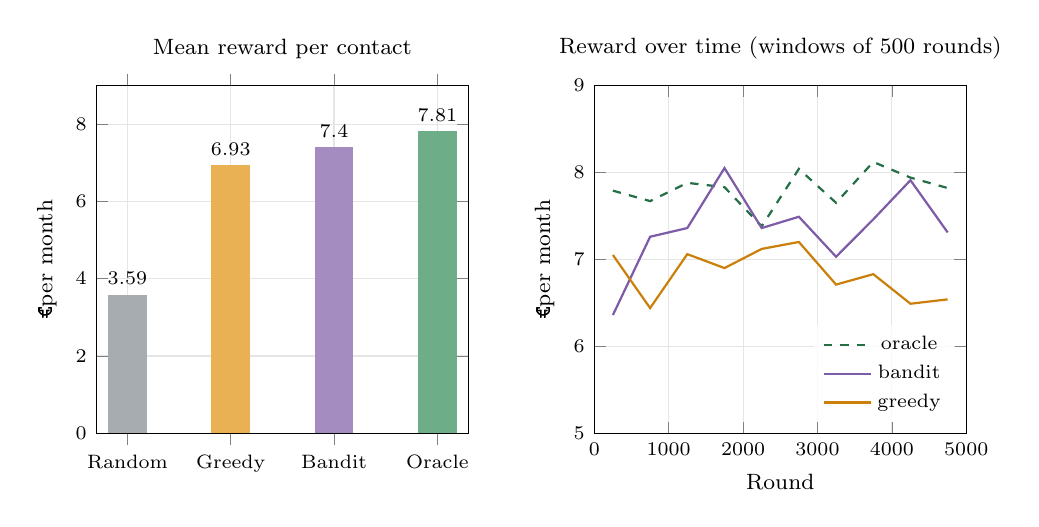
\begin{tikzpicture}
\begin{groupplot}[group style={group size=2 by 1,horizontal sep=1.6cm},width=0.52\linewidth,height=6cm]
\nextgroupplot[title={Mean reward per contact},ybar,bar width=14pt,symbolic x coords={Random,Greedy,Bandit,Oracle},xtick={Random,Greedy,Bandit,Oracle},
  ylabel={\eur per month},ymin=0,ymax=9,nodes near coords,every node near coord/.append style={font=\scriptsize},point meta=y,/pgf/number format/.cd,fixed,precision=2]
\addplot[fill=cg!60,draw=none,bar shift=0pt] coordinates {(Random,3.59)};
\addplot[fill=ca!70,draw=none,bar shift=0pt] coordinates {(Greedy,6.93)};
\addplot[fill=cp!70,draw=none,bar shift=0pt] coordinates {(Bandit,7.40)};
\addplot[fill=ct!70,draw=none,bar shift=0pt] coordinates {(Oracle,7.81)};
\nextgroupplot[title={Reward over time (windows of 500 rounds)},xlabel={Round},ylabel={\eur per month},xmin=0,xmax=5000,ymin=5,ymax=9,
  legend style={at={(0.97,0.03)},anchor=south east},xtick={0,1000,...,5000},xticklabel style={/pgf/number format/1000 sep={}}]
\addplot[no markers,thick,ct!80!black,dashed] coordinates {(250,7.79)(750,7.67)(1250,7.88)(1750,7.83)(2250,7.38)(2750,8.04)(3250,7.65)(3750,8.12)(4250,7.94)(4750,7.82)};
\addplot[no markers,thick,cp,mark=*,mark size=1.3pt] coordinates {(250,6.36)(750,7.26)(1250,7.36)(1750,8.05)(2250,7.36)(2750,7.49)(3250,7.03)(3750,7.46)(4250,7.91)(4750,7.31)};
\addplot[no markers,thick,ca!90!black] coordinates {(250,7.05)(750,6.44)(1250,7.06)(1750,6.9)(2250,7.12)(2750,7.2)(3250,6.71)(3750,6.83)(4250,6.49)(4750,6.54)};
\legend{oracle,bandit,greedy}
\end{groupplot}
\end{tikzpicture}
\caption{Offline replay of 5\,000 contacts. The bandit reaches 94.7\,\% of the oracle (the best \emph{expected} reward,
unknowable in practice), beats greedy-by-value by 6.7\,\% and random by 2.1$\times$. On the right, the bandit starts below greedy
(it is still exploring: \eur 6.36 in the first 500 rounds) then catches up and overtakes it. Individual windows are noisy (500 draws each), so read the trend, not single points.}
\end{figure}

\begin{figure}[h]
\centering
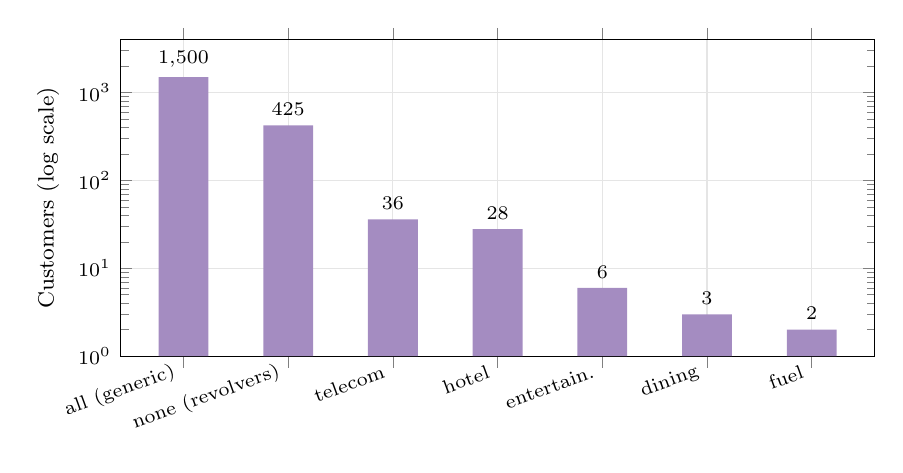
\begin{tikzpicture}
\begin{axis}[base,height=5.6cm,ybar,bar width=18pt,symbolic x coords={all,none,telecom,hotel,entertainment,dining,fuel},xtick=data,
  xticklabels={all (generic),none (revolvers),telecom,hotel,entertain.,dining,fuel},xticklabel style={rotate=20,anchor=east,font=\scriptsize},
  ymode=log,ymin=1,ymax=4000,ylabel={Customers (log scale)},nodes near coords,point meta=rawy,every node near coord/.append style={font=\scriptsize},log origin=infty]
\addplot[fill=cp!70,draw=none] coordinates {(all,1500)(none,425)(telecom,36)(hotel,28)(entertainment,6)(dining,3)(fuel,2)};
\end{axis}
\end{tikzpicture}
\caption{Final recommendation for each of the 2\,000 customers (after training the bandit for 20\,000 simulated rounds, then choosing greedily from the posterior mean). 425 revolvers receive ``none'' by rule; 1\,500 of the 1\,575 offers (95\,\%) are the generic \emph{all purchases} cash-back; only 75 are sector-specific.}
\label{fig:reco}
\end{figure}

\begin{warnbox}
\textbf{Reading Figure~\ref{fig:reco} honestly.} The bandit is not broken: for most customers, the generic cash-back hits its \eur 20 cap
(median recommended value is exactly \eur 20), which beats every sector-specific benefit in \eur terms and has a respectable simulated acceptance. The real finding is that
\emph{with this catalog, a single generic benefit dominates}. More variety would need either richer sector benefits (higher caps/rates) or real acceptance data in which
sector-specific offers convert better than the simulator assumes.
\end{warnbox}

\why{
\begin{itemize}
\item \textbf{Bandit, not a ranker}: there is no labelled history of ``offer X shown, outcome Y''. A bandit learns \emph{online} and keeps exploring, and the same code can consume real logged outcomes when they exist (swap the environment function).
\item \textbf{Thompson Sampling} is simple, has no tuning of explore/exploit schedules, and uses a uncertainty-aware posterior per arm.
\item \textbf{Linear in the context}: transparent coefficients, fast updates, and natural use of CATE and segment as features.
\item \textbf{Hard guard for revolvers}: the harm of an offer to a sleeping dog is not something to leave to an exploration policy.
\end{itemize}}

% =====================================================================
\section{Step 7 --- ``Claire'': writing the message and checking it}
% =====================================================================

\subsection{From recommendation to fact sheet}

For each selected customer, a deterministic function builds a short list of plain-sentence \emph{facts} (the only numbers the model may use)
and a persona summary. Example for customer 684:

\begin{msg}[ca]{Fact sheet passed to the model (user 684)}
\upshape\ttfamily\footnotesize
- Recommended benefit: 1\% cash-back on all purchases, up to \eur20/month (premium card)\\
- Their total card spend: \eur2,720/month\\
- Value to them: \eur20/month (\eur240/year)\\
- Premium card fee: \eur240/year\\
- Net gain of premium over standard, after the fee: \eur70/month\\[3pt]
persona: tone = concise\_data; motivation = savings; digital = low; channel = phone; language = French
\end{msg}

\subsection{The prompt: rules the writer must obey}

\begin{center}
\small
\begin{tabularx}{\linewidth}{@{}p{0.6cm}p{5.4cm}X@{}}
\toprule
\textbf{\#} & \textbf{Rule in the prompt} & \textbf{Reason}\\
\midrule
1 & Write only in the customer's language & EN / FR; mixed-language messages feel broken\\
2 & Greeting first (``Hi'', ``Bonjour'', \dots), no invented name & the bank does not know the name; inventing one is worse than none\\
3 & Last line exactly \texttt{Claire} & consistent, checkable sign-off\\
4 & Always \texttt{\eur}, never ``EUR'', ``euros'', \texttt{\$} & regulatory and brand consistency\\
5 & Only numbers in the facts (monthly $\to$ yearly allowed) & no hallucinated figures; the most important rule\\
6 & Respect the channel and its character limit & SMS 320, push 180, in-app 400, phone 800, email 1\,200\\
7 & No promises of approval or guaranteed returns & compliance\\
\bottomrule
\end{tabularx}
\end{center}

The persona then sets the \emph{tone}, the \emph{motivation} to frame around, and the \emph{digital level} (plainer words, less jargon for low digital).

\subsection{The agent: write, score, retry, flag}

\begin{figure}[h]
\centering
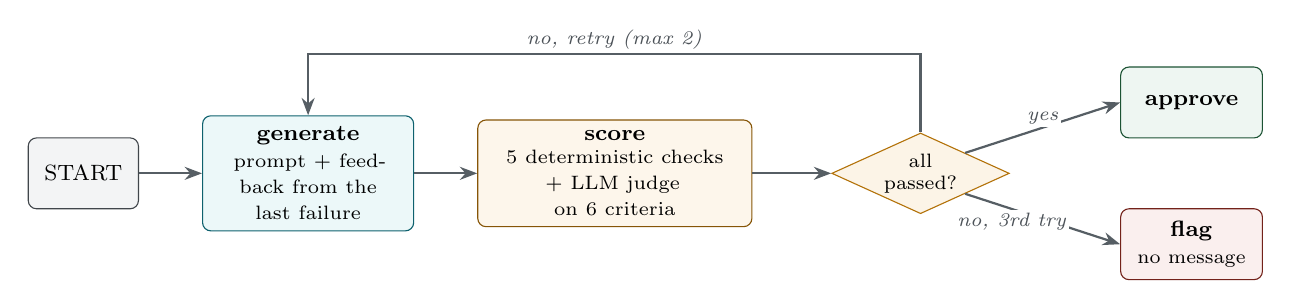
\begin{tikzpicture}[node distance=8mm]
\node[wide=cg,minimum width=1.4cm] (st) {START};
\node[wide=ck,right=of st,text width=2.4cm] (gen) {\textbf{generate}\\\scriptsize prompt $+$ feedback from the last failure};
\node[wide=ca,right=of gen,text width=3.2cm] (sc) {\textbf{score}\\\scriptsize 5 deterministic checks\\\scriptsize $+$ LLM judge on 6 criteria};
\node[dec,right=of sc,xshift=2mm] (rt) {all\\passed?};
\node[wide=ct,right=14mm of rt,yshift=9mm,minimum width=1.8cm] (ap) {\textbf{approve}};
\node[wide=cr,right=14mm of rt,yshift=-9mm,minimum width=1.8cm] (fl) {\textbf{flag}\\\scriptsize no message};
\draw[flow] (st)--(gen); \draw[flow] (gen)--(sc); \draw[flow] (sc)--(rt);
\draw[flow] (rt.north east)--node[above,lab,pos=0.5]{yes}(ap.west);
\draw[flow] (rt.south east)--node[below,lab,pos=0.3]{no, 3rd try}(fl.west);
\draw[flow] (rt.north) -- ++(0,1.0) -| node[above,lab,pos=0.25]{no, retry (max 2)} (gen.north);
\end{tikzpicture}
\caption{LangGraph state machine. A failed draft is fed back with the exact failed criteria and their reasons. At most 3 attempts in total; after that the customer gets \emph{no message} rather than a bad one.}
\end{figure}

\subsection{Two layers of quality gate}

\begin{center}
\small
\begin{tabularx}{\linewidth}{@{}p{3.6cm}p{2cm}X@{}}
\toprule
\textbf{Check} & \textbf{Type} & \textbf{What it enforces}\\
\midrule
\code{currency} & regex & no EUR / euros / USD / \texttt{\$}\\
\code{greeting} & regex & first line starts with a greeting of the target language\\
\code{signature} & regex & last line contains ``Claire''\\
\code{numbers} & parser & every number appears in the facts (or $\times12$); handles \texttt{1,234.50} and \texttt{1\,234,50}\\
\code{length} & count & within the channel's character limit\\
\midrule
\code{tone_match}, \code{motivation_framing} & LLM judge & persona fit\\
\code{channel_fit}, \code{language_correct} & LLM judge & format/length for channel and digital level; fully in the target language\\
\code{clarity}, \code{no_overpromise} & LLM judge & value is understandable; no pressure, guarantees or claims beyond the facts\\
\bottomrule
\end{tabularx}
\end{center}
A message passes only if \emph{all} five checks hold and every judge score is $\geq 4/5$.

\why{
\begin{itemize}
\item \textbf{Deterministic checks first-class}: compliance properties (currency, no invented numbers, signature) must never depend on an LLM's mood. They are cheap, exact and testable (the test-suite exercises each with fake models).
\item \textbf{LLM judge for the fuzzy parts}: tone, framing and language quality cannot be regex'd.
\item \textbf{Specific feedback on retry}: telling the writer exactly which criterion failed and why converges faster than ``try again''.
\item \textbf{Flag instead of send}: a missing message is cheap; a wrong one in a regulated setting is not.
\item \textbf{Writer temperature 0.7, judge temperature 0}: creative drafts, repeatable scoring.
\end{itemize}}

\subsection{What the 25 messages looked like}

\begin{figure}[h]
\centering
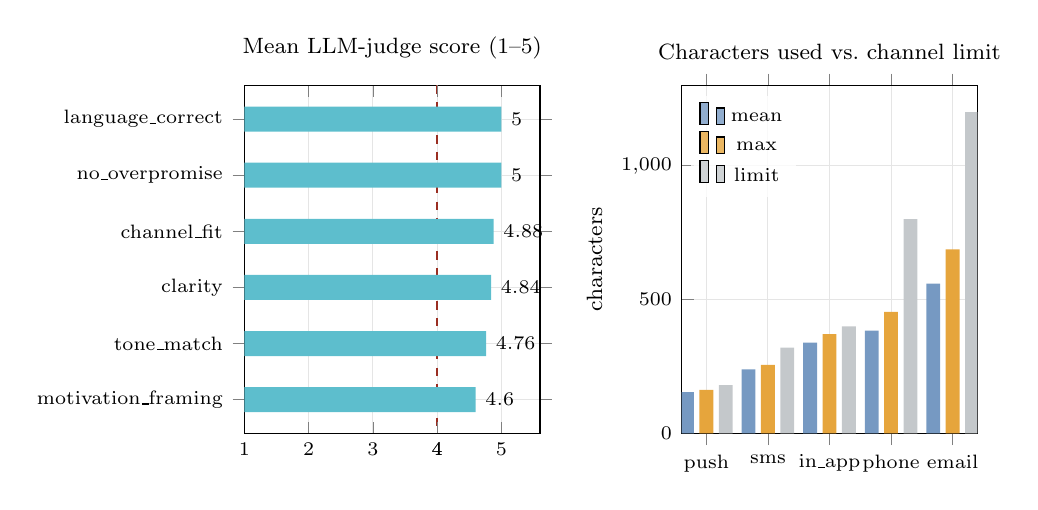
\begin{tikzpicture}
\begin{groupplot}[group style={group size=2 by 1,horizontal sep=1.8cm},width=0.44\linewidth,height=6cm]
\nextgroupplot[title={Mean LLM-judge score (1--5)},xbar,bar width=9pt,symbolic y coords={language\_correct,no\_overpromise,channel\_fit,clarity,tone\_match,motivation\_framing},
  ytick=data,y dir=reverse,xmin=1,xmax=5.6,xtick={1,2,3,4,5},extra x ticks={4},extra x tick style={grid=major,grid style={dashed,cr!80!black,thick}},nodes near coords,every node near coord/.append style={font=\scriptsize},
  point meta=x,/pgf/number format/.cd,fixed,precision=2,enlarge y limits=0.12]
\addplot[fill=ck!70,draw=none] coordinates {(5.00,language\_correct)(5.00,no\_overpromise)(4.88,channel\_fit)(4.84,clarity)(4.76,tone\_match)(4.60,motivation\_framing)};

\nextgroupplot[title={Characters used vs.\ channel limit},ybar,bar width=5pt,symbolic x coords={push,sms,in\_app,phone,email},xtick=data,
  ymin=0,ymax=1300,ylabel={characters},legend style={at={(0.03,0.97)},anchor=north west}]
\addplot[fill=cb!70,draw=none] coordinates {(push,154)(sms,239)(in\_app,339)(phone,384)(email,559)};
\addplot[fill=ca!80,draw=none] coordinates {(push,162)(sms,256)(in\_app,371)(phone,454)(email,687)};
\addplot[fill=cg!40,draw=none] coordinates {(push,180)(sms,320)(in\_app,400)(phone,800)(email,1200)};
\legend{mean,max,limit}
\end{groupplot}
\end{tikzpicture}
\caption{Left: judge scores averaged over the 25 messages (all attempts were first attempts; dashed line = pass threshold of 4).
Motivation framing is the weakest criterion (4.60). Right: length used vs.\ the channel limit: the model respects the tight channels
(push uses at most 162 of 180 characters).}
\end{figure}

\begin{center}
\small
\begin{tabular}{@{}lrrrrr|r@{}}
\toprule
 & \textbf{phone} & \textbf{push} & \textbf{email} & \textbf{in-app} & \textbf{SMS} & \textbf{Total}\\
\midrule
English & 3 & 3 & 3 & 3 & 3 & 15\\
French & 4 & 1 & 2 & 2 & 1 & 10\\
\midrule
Total & 7 & 4 & 5 & 5 & 4 & 25\\
\bottomrule
\end{tabular}
\captionof{table}{Composition of the generated set: 5 channels $\times$ 2 languages, all approved at attempt 1; 20 baseline customers and 5 transactors (revolvers receive no message by design).}
\end{center}

Four examples, from different channels, languages and personas:

\begin{msg}[ck]{User 1699 --- push, English, tone: exclusive, motivation: status, hotel benefit (net gain \eur 88/month)}
Hello,\\
With your premium card, you earn €40/month cash-back on hotel stays, netting you €88/month after the fee. Enjoy the perks of exclusivity!\\
Claire
\end{msg}

\begin{msg}[ck]{User 936 --- SMS, English, tone: friendly, motivation: security, digital: low (phone plan benefit)}
Hello!\\
With your premium card, you get a phone plan included worth €20/month. That adds up to €240 a year, giving you a nice net gain of €53/month after the fee. It's a great way to keep your spending secure!\\
Claire
\end{msg}

\begin{msg}[ck]{User 324 --- in-app, French, tone: reassuring, motivation: status (hotel benefit)}
Bonjour,\\
Saviez-vous que votre carte premium vous permet de bénéficier de 5\% de cash-back sur vos dépenses d'hôtel ? Avec vos 952 € par mois, cela représente 40 € de retour chaque mois, soit 480 € par an ! Après la cotisation annuelle de 240 €, vous gagnez encore 44 € par mois. C'est une belle façon d'optimiser votre statut tout en réalisant des économies.\\
Claire
\end{msg}

\begin{msg}[ck]{User 684 --- phone, French, tone: concise data, motivation: savings, digital: low (generic cash-back)}
Bonjour,\\
Avec votre carte premium, vous bénéficiez d'un cash-back de 1\% sur tous vos achats, ce qui vous rapporte 20 € par mois, soit 240 € par an. Après la cotisation de 240 € pour la carte, vous avez un gain net de 70 € chaque mois. Cela représente une belle économie pour vous !\\
Claire
\end{msg}

% =====================================================================
\section{Results across the funnel}
% =====================================================================

\begin{figure}[H]
\centering
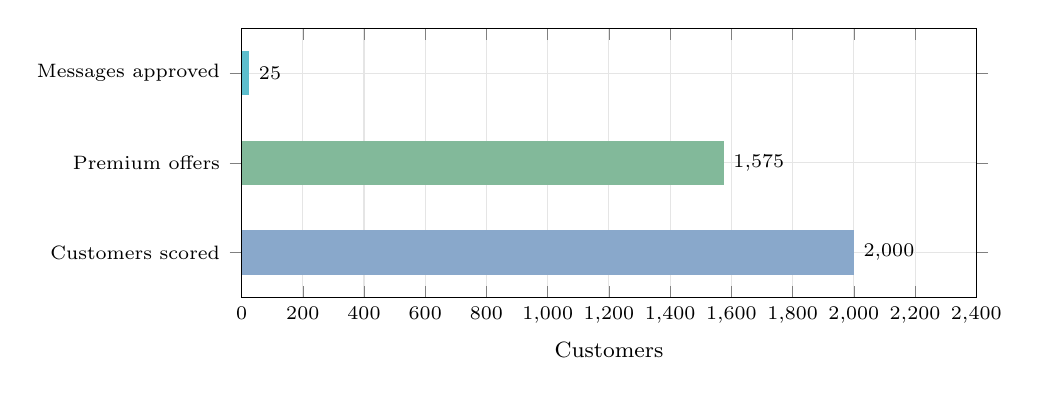
\begin{tikzpicture}
\begin{axis}[width=0.9\linewidth,height=5cm,xbar,bar width=16pt,symbolic y coords={Messages approved,Premium offers,Customers scored},
  ytick={Customers scored,Premium offers,Messages approved},y dir=reverse,xmin=0,xmax=2400,nodes near coords,every node near coord/.append style={font=\scriptsize},enlarge y limits=0.25,xlabel={Customers}]
\addplot[fill=cb!60,draw=none,bar shift=0pt] coordinates {(2000,Customers scored)};
\addplot[fill=ct!60,draw=none,bar shift=0pt] coordinates {(1575,Premium offers)};
\addplot[fill=ck!70,draw=none,bar shift=0pt] coordinates {(25,Messages approved)};
\end{axis}
\end{tikzpicture}
\caption{Funnel. The gap between 2\,000 and 1\,575 is the 425 revolvers deliberately excluded. The 25 messages are a demonstration sample, not the whole 1\,575.}
\end{figure}

\paragraph{Summary by segment.}
\begin{center}
\small
\setlength{\tabcolsep}{4pt}\begin{tabular}{@{}lrrrrl@{}}
\toprule
\textbf{Segment} & \textbf{Cust.} & \textbf{Spend/mo} & \textbf{True $\tau$} & \textbf{Est.\ CATE} & \textbf{Action}\\
\midrule
baseline & 1\,207 & \eur 3\,120 & $+0.130$ & $+0.167$ & premium offer\\
transactor & 368 & \eur 4\,096 & $+0.170$ & $+0.175$ & premium offer, travel benefits\\
revolver & 425 & \eur 7\,596 & $-0.125$ & $-0.139$ & \textbf{none} (sleeping dogs)\\
\bottomrule
\end{tabular}
\end{center}

% =====================================================================
\section{Limitations and what I would change}
\label{sec:limits}
% =====================================================================

\subsection{What is simulated, and what that implies}

\begin{center}
\small
\begin{tabularx}{\linewidth}{@{}p{3cm}p{4.6cm}X@{}}
\toprule
\textbf{Component} & \textbf{Currently} & \textbf{With real data}\\
\midrule
Transactions & IBM TabFormer, itself synthetic & real card data; same code\\
Upgrade campaign & simulated randomised trial, known $\tau$ & replace with logged campaign outcomes; evaluate with a held-out Qini curve\\
Personas & seeded draws conditioned on behaviour & fit weights on engagement / opt-in data\\
Offer acceptance & logistic model with random affinities & feed logged accept/decline into the bandit instead of the simulator\\
Benefit catalog & illustrative rates and caps & actual product terms\\
\bottomrule
\end{tabularx}
\end{center}

\subsection{Findings from the run that deserve attention}

\begin{warnbox}
\begin{enumerate}[leftmargin=14pt]
\item \textbf{Some offers lose money for the customer.} 63 of the 1\,575 premium offers (4.0\,\%) have a negative net gain after the \eur 240 fee, and in the 25-message sample it is 8 of 25 (32\,\%; the sample is not a uniform draw: only 10 of 25 are generic cash-back, against 95\,\% in the population). Messages for these customers lead with a real benefit but cannot honestly claim overall savings. \emph{Fix: gate offers on upgrade\_gain $>$ 0, or switch to a standard-tier offer.}
\item \textbf{The number check validates presence, not meaning.} For user 1699 the message says \texttt{\eur40/month cash-back on hotel stays, netting you \eur88/month after the fee}, which reads as if \eur40 became \eur88; \eur88 is actually the net gain of the whole premium card, a different fact. Both numbers are in the fact sheet, so the checker passes it and the judge did not object. \emph{Fix: derive complete sentence templates for each number, or ask the judge specifically about number semantics.}
\item \textbf{The retry loop was never exercised live.} All 25 messages were approved on attempt 1. That can mean a good writer, but also a lenient judge: by default the writer and the judge are the same model (\code{openai/gpt-4o-mini} unless overridden), and the judge's lowest mean score is 4.60. The retry/flag path is covered by unit tests with fake models, but not yet proven under a real failure. \emph{Fix: a different (stronger) judge model, plus a deliberate set of adversarial test cases.}
\item \textbf{Recommendation diversity is low.} 95\,\% of offers are the generic cash-back (Figure~\ref{fig:reco}) because it hits its \eur 20 cap for nearly everyone. That is a catalog property, not a bug, but it limits personalisation of \emph{what} is offered; personalisation is then carried mostly by \emph{how} it is said.
\item \textbf{Uplift evaluation is optimistic.} The CATE is scored on the same 2\,000 customers it was fit on, against a simulator written by the same author. The 0.75 correlation shows the method recovers a known truth; it does not validate the real-world effect.
\item \textbf{Segmentation keeps 52.7\,\% of the variance} (4 components). It is sufficient for three well-separated groups, but the 11-feature space was not tuned further.
\end{enumerate}
\end{warnbox}

\subsection{Next steps, in order of value}
\begin{enumerate}
\item Gate on net gain; add a ``fee exceeds benefit'' branch to the fact sheet.
\item Use a separate judge model and run a red-team set to exercise retry and flag.
\item Replace the three simulators with real campaign, contact-preference and acceptance logs; keep the interfaces.
\item Add a held-out Qini / uplift curve and bandit off-policy evaluation (inverse propensity weighting) on real logs.
\item Enrich the benefit catalog (sector caps/rates) so the bandit has genuinely different options to choose from.
\end{enumerate}

% =====================================================================
\section{Reproducing the run}
% =====================================================================

\begin{center}
\small
\begin{tabular}{@{}p{7.2cm}p{8.3cm}@{}}
\toprule
\textbf{Command} & \textbf{Effect}\\
\midrule
\code{uv run python -m reco ingest} & CSV $\to$ Parquet warehouse (heavy; ran on a CPU pod)\\
\code{uv run python -m reco train} & features, segments, personas, uplift, valuation, bandit; writes \code{user\_scores}, \code{personas}, \code{user\_benefit\_value}, \code{user\_reco}\\
\code{uv run pytest} & unit tests (pipeline, serving, messaging with fake models)\\
\code{source .env; uv run python -m messaging 12 57} & writes messages for the given users (or \code{--sample N}); appends to \code{data/messages.parquet}\\
\bottomrule
\end{tabular}
\end{center}

\subsection*{Key parameters}
\begin{center}
\small
\begin{tabular}{@{}llp{7.8cm}@{}}
\toprule
\textbf{Stage} & \textbf{Parameter} & \textbf{Value}\\
\midrule
Segmentation & PCA / $k$ search / n\_init / seed & 4 components / 3--6 / 10 / 0\\
Uplift & campaign treatment prob.\ / learner & 0.5 / gradient boosting, depth 3 (4 models)\\
Value & premium fee & \eur 240 per year\\
Bandit & arms / context dim.\ / top-$K$ / $v$ & 16 / 8 / 3 / 0.3\\
Bandit & evaluation / final training rounds & 5\,000 / 20\,000\\
Acceptance model & $\alpha,\beta,\gamma$ & $-2.0,\ 1.5,\ 1.0$\\
Messaging & attempts / judge threshold & 3 (draft $+$ 2 retries) / $\geq 4$ on each of 6 criteria\\
Messaging & writer / judge temperature & 0.7 / 0\\
\bottomrule
\end{tabular}
\end{center}

% =====================================================================
\appendix
\section{The 25 generated messages at a glance}
% =====================================================================

\begin{center}
\scriptsize
\setlength{\tabcolsep}{3.2pt}
\newcommand{\red}[1]{\textcolor{cr}{#1}}
\begin{tabular}{@{}rllllllrrr@{}}
\toprule
\textbf{User} & \textbf{Segment} & \textbf{Channel} & \textbf{Lang.} & \textbf{Tone} & \textbf{Motivation} & \textbf{Benefit sector} & \textbf{Value} & \textbf{Net gain} & \textbf{Chars}\\
\midrule
1604 & baseline & SMS & EN & exclusive & convenience & all & 20.0 & 34.5 & 241\\
324 & transactor & in-app & FR & reassuring & status & hotel & 40.0 & 43.7 & 371\\
209 & baseline & phone & EN & friendly & savings & telecom & 20.0 & 48.6 & 405\\
544 & baseline & email & EN & concise data & security & all & 20.0 & 25.6 & 502\\
231 & baseline & push & EN & reassuring & savings & entertainment & 7.4 & \red{$-$18.6} & 148\\
542 & baseline & push & EN & exclusive & status & dining & 1.0 & \red{$-$18.3} & 152\\
1350 & baseline & email & FR & reassuring & status & fuel & 1.4 & \red{$-$17.8} & 549\\
156 & transactor & phone & FR & exclusive & status & all & 20.0 & 53.0 & 362\\
1239 & baseline & SMS & EN & friendly & security & all & 20.0 & \red{$-$3.7} & 256\\
1304 & baseline & push & FR & friendly & security & all & 20.0 & 37.7 & 162\\
1775 & baseline & phone & EN & reassuring & security & all & 20.0 & 32.3 & 454\\
1469 & baseline & email & FR & reassuring & savings & all & 10.1 & 8.5 & 494\\
684 & baseline & phone & FR & concise data & savings & all & 20.0 & 69.8 & 294\\
768 & baseline & in-app & EN & reassuring & security & all & 20.0 & 70.5 & 365\\
1597 & baseline & in-app & FR & reassuring & security & all & 20.0 & 66.5 & 359\\
1484 & baseline & SMS & FR & friendly & savings & dining & 5.4 & \red{$-$13.2} & 239\\
936 & baseline & SMS & EN & friendly & security & telecom & 20.0 & 53.0 & 219\\
1639 & baseline & in-app & EN & concise data & savings & entertainment & 7.3 & \red{$-$17.3} & 272\\
221 & baseline & email & EN & reassuring & security & telecom & 20.0 & 5.0 & 562\\
810 & baseline & phone & FR & concise data & savings & telecom & 20.0 & 4.2 & 364\\
457 & baseline & email & EN & reassuring & security & entertainment & 6.0 & \red{$-$19.5} & 687\\
1699 & transactor & push & EN & exclusive & status & hotel & 40.0 & 88.4 & 155\\
453 & transactor & in-app & EN & exclusive & status & hotel & 36.4 & 94.1 & 328\\
911 & transactor & phone & FR & friendly & convenience & hotel & 36.4 & 94.4 & 446\\
1817 & baseline & phone & EN & friendly & convenience & fuel & 0.5 & \red{$-$19.0} & 366\\
\bottomrule
\end{tabular}
\end{center}

\small Value and net gain are in \eur per month. Red: the premium card costs more than it returns on this customer's spend.
Note that one persona draw can look inconsistent (e.g.\ user 324: motivation \emph{status} with a \emph{reassuring} tone) because traits are sampled
\emph{probabilistically}, never deterministically; the agent honours whichever combination it is given.

\end{document}
